\chapter{Operations and Periodicity}
\label{chap:period_foundation}

\markboth{Periodic Foundations}{Periodic Foundations}

\begin{remark}[Positioning of this chapter and the two logical chains]\label{rem:chapter_positioning}
The root of periodicity is invariance under transformations. This chapter takes iteration as the starting point of every concept, examines one by one the true logical direction of each arrow and the conditions under which it holds. The core conclusion is: within the purely algebraic framework of this chapter, a finite-order action is the direct sufficient and necessary condition for obtaining uniform periodicity and closed orbits; conservation and symmetry are auxiliary tools for \textbf{discovering} finite order, not a necessary link in the existence of periodicity.

Thus the chapter distinguishes two chains:
\[
\boxed{\text{Core criterion chain: finite-order action}\Longrightarrow\text{closed orbit}\Longrightarrow\text{period}}
\]
\[
\boxed{\text{Auxiliary discovery chain: conservation}\longleftarrow\text{symmetry}\quad\text{(used to discover finite order)}}
\]
The core criterion chain is sufficient and necessary in the bijective framework; the auxiliary discovery chain is heuristic, and its direction is often reversed. Specifically:
\begin{itemize}
    \item symmetry $\Rightarrow$ conservation (with conditions), but not conservation $\Rightarrow$ symmetry;
    \item period $\Rightarrow$ symmetry (the evolution group itself is a finite cyclic group), yet period $\nRightarrow$ non-trivial conservation;
    \item the conjunction of symmetry and conservation still $\nRightarrow$ period.
\end{itemize}

This chapter uses mainly the algebraic language of set theory, group theory and group representation theory; notions involving topology (bounded, dense, compact) are used only as heuristic illustrations.
\end{remark}

\section{Foundations of group theory and group actions}
\label{sec:group_theory}

This section builds, in a self-contained way, the group-theoretic language required in this chapter: groups, subgroups, homomorphisms, quotient groups, the order of an element, the torsion subgroup, cyclic groups, group actions, orbits and stabilisers. The notation is fixed in this section and used throughout the chapter.

\subsection{Groups, subgroups and homomorphisms}

\begin{definition}[Group]\label{def:group}
A \textbf{group} is an ordered pair $(G,\cdot)$, where $G$ is a non-empty set and $\cdot:G\times G\to G$ is a binary operation satisfying:
\begin{enumerate}[label=(\arabic*)]
    \item \textbf{Closure}: for all $a,b\in G$, $a\cdot b\in G$;
    \item \textbf{Associativity}: for all $a,b,c\in G$, $(a\cdot b)\cdot c=a\cdot(b\cdot c)$;
    \item \textbf{Identity element}: there exists $e\in G$ such that $e\cdot a=a\cdot e=a$ for all $a\in G$;
    \item \textbf{Inverse element}: for every $a\in G$ there exists $a^{-1}\in G$ such that $a\cdot a^{-1}=a^{-1}\cdot a=e$.
\end{enumerate}
\end{definition}

\begin{definition}[Abelian group]\label{def:abelian_group}
A group $(G,\cdot)$ is called an \textbf{Abelian group} (or commutative group) if, for all $a,b\in G$,
\[
a\cdot b=b\cdot a.
\]
The operation of an Abelian group is often written additively as $+$, the identity element is written $0$ and the inverse as $-a$; in this notation the power rule is written as the multiple rule $n(a+b)=na+nb$.
\end{definition}

\begin{example}[Three fundamental Abelian groups]\label{ex:three_abelian_groups}
The following three Abelian groups are the algebraic carriers of the transformation theory of this chapter:
\begin{enumerate}[label=(\roman*)]
    \item \textbf{The additive group of integers} $(\mathbb{Z},+)$: identity element $0$, inverse of $a$ equal to $-a$. This is the algebraic basis of discrete translation.
    \item \textbf{The multiplicative group of positive reals} $(\mathbb{R}^+,\times)$: identity element $1$, inverse of $a$ equal to $1/a$. This is the algebraic basis of scaling.
    \item \textbf{The circle group} $U(1)=\{z\in\mathbb{C}\mid |z|=1\}$ (under multiplication of complex numbers): identity element $1$, inverse of $z$ equal to $\bar z$. Its operation is the multiplication of complex powers
    \[
    e^{i\theta}\cdot e^{i\phi}=e^{i(\theta+\phi)}.
    \]
    This is the algebraic basis of rotation.
\end{enumerate}
All three are Abelian groups; but their \textbf{torsion structure} is utterly different, and this difference will become the focus of the theory of periodicity in Theorem \ref{thm:order_structure}.
\end{example}

\begin{definition}[Subgroup]\label{def:subgroup}
Let $G$ be a group and let $H\subseteq G$ be non-empty. If $H$ itself forms a group under the operation of $G$, then $H$ is called a \textbf{subgroup} of $G$, written $H\le G$.
\end{definition}

\begin{proposition}[Subgroup criterion]\label{prop:subgroup_criterion}
Let $G$ be a group and let $H\subseteq G$ be non-empty. Then $H\le G$ if and only if:
\begin{enumerate}[label=(\roman*)]
    \item for all $a,b\in H$, $ab\in H$;
    \item for all $a\in H$, $a^{-1}\in H$.
\end{enumerate}
Equivalently, $H\le G$ if and only if $ab^{-1}\in H$ for all $a,b\in H$.
\end{proposition}

\begin{proof}
Necessity: if $H$ is a subgroup, then closure (i) and closure under inverses (ii) follow directly from the definition of a subgroup. Sufficiency: closure follows from (i), and associativity is inherited from $G$. From (ii) and (i), taking $a\in H$ gives $aa^{-1}=e\in H$, so the identity element exists; the inverse is given by (ii). The equivalent criterion follows directly from $b^{-1}\in H$ and $ab^{-1}\in H$.
\end{proof}

\begin{definition}[Group homomorphisms and isomorphisms]\label{def:homomorphism}
Let $G,H$ be groups. A map $\varphi:G\to H$ is called a \textbf{group homomorphism} if
\[
\varphi(ab)=\varphi(a)\varphi(b),\qquad \forall a,b\in G.
\]
If $\varphi$ is a bijection, it is called a \textbf{group isomorphism}, written $G\cong H$. The \textbf{kernel} and \textbf{image} of a homomorphism $\varphi$ are respectively
\[
\ker\varphi=\{g\in G\mid \varphi(g)=e_H\},\qquad
\operatorname{im}\varphi=\{\varphi(g)\mid g\in G\}.
\]
\end{definition}

\begin{definition}[Normal subgroups and quotient groups]\label{def:normal_subgroup}
Let $N\le G$. If $gN=Ng$ for all $g\in G$, then $N$ is called a \textbf{normal subgroup} of $G$, written $N\trianglelefteq G$. In this case the set of cosets
\[
G/N=\{gN\mid g\in G\}
\]
forms a group under the operation $(gN)(hN)=(gh)N$, called the \textbf{quotient group}.
\end{definition}

\begin{theorem}[Fundamental theorem of homomorphisms]\label{thm:first_isomorphism}
Let $\varphi:G\to H$ be a group homomorphism. Then
\[
G/\ker\varphi\cong \operatorname{im}\varphi.
\]
In particular, $\ker\varphi\trianglelefteq G$.
\end{theorem}

\begin{proof}
Let $K=\ker\varphi$. For any $g\in G$, define $\bar\varphi(gK)=\varphi(g)$. If $gK=hK$, then $h^{-1}g\in K$, so $\varphi(h^{-1}g)=e$, whence $\varphi(g)=\varphi(h)$, and the map is well defined. The homomorphism property follows directly from that of $\varphi$. The kernel is $K$, so the map is injective; the image is $\operatorname{im}\varphi$, so the map is surjective onto the image. Hence $G/K\cong \operatorname{im}\varphi$.
\end{proof}

\begin{figure}[htbp]
\centering
\begin{tikzpicture}[>=stealth, node distance=2.8cm]
    \node (G) {$G$};
    \node[right=of G] (H) {$H$};
    \node[below=of G] (Q) {$G/\ker\varphi$};
    \node[below=of H] (I) {$\operatorname{im}\varphi$};

    \draw[->, thick] (G) -- node[above] {$\varphi$} (H);
    \draw[->, thick] (G) -- node[left] {$\pi$} (Q);
    \draw[->, thick] (Q) -- node[below] {$\cong$} (I);
    \draw[->, thick] (I) -- node[right] {$\iota$} (H);

    \node[font=\footnotesize, below=0.7cm of Q, align=center]
        {$\pi$: natural projection\\ $\iota$: inclusion map};
\end{tikzpicture}
\caption{Fundamental theorem of homomorphisms: $G/\ker\varphi\cong\operatorname{im}\varphi$. Every homomorphism $\varphi$ can be factored as `projection---isomorphism---inclusion'.}
\label{fig:first_isomorphism}
\end{figure}

\begin{definition}[Centraliser]\label{def:centraliser}
Let $G$ be a group and $S\subseteq G$. The \textbf{centraliser} of $S$ in $G$ is
\[
C_G(S)=\{g\in G\mid gs=sg,\ \forall s\in S\}.
\]
The \textbf{centre} of $G$ is $Z(G)=C_G(G)$.
\end{definition}

\begin{proposition}[The centraliser is a subgroup]\label{prop:centraliser_subgroup}
For any $S\subseteq G$, one has $C_G(S)\le G$, and $Z(G)\trianglelefteq G$.
\end{proposition}

\begin{proof}
$e\in C_G(S)$. If $a,b\in C_G(S)$, then for any $s\in S$,
\[
(ab)s=a(bs)=a(sb)=(as)b=(sa)b=s(ab),
\]
so $ab\in C_G(S)$. Also $as=sa$ implies $a^{-1}s=sa^{-1}$, so $a^{-1}\in C_G(S)$. The subgroup criterion gives $C_G(S)\le G$. The centre is analogous.
\end{proof}

\begin{property}[Power rule for Abelian groups]\label{prop:abelian_power}
Let $G$ be an Abelian group, $a,b\in G$ and $n\in\mathbb{Z}$. Then
\[
(ab)^n=a^n b^n.
\]
\end{property}

\begin{proof}
First suppose $n\ge 0$ and argue by induction on $n$. For $n=0$: $(ab)^0=e=ee=a^0b^0$. Suppose $(ab)^n=a^n b^n$; then
\[
(ab)^{n+1}=(ab)^n(ab)=a^n b^n a b=a^n a b^n b=a^{n+1}b^{n+1},
\]
where the third step uses the commutative law $b^n a=a b^n$. For $n<0$,
\[
(ab)^n=((ab)^{-1})^{-n}=(a^{-1}b^{-1})^{-n}=(a^{-1})^{-n}(b^{-1})^{-n}=a^n b^n.
\]
\end{proof}

\begin{remark}[The necessity of commutativity]\label{rem:abelian_power_necessary}
The power rule $(ab)^n=a^n b^n$ generally fails in a non-Abelian group: $(ab)^2=abab$ and $a^2b^2=aabb$ are equal if and only if $ba=ab$. The commutative law is precisely the condition that `two iterations may be performed in either order'.
\end{remark}

\subsection{Order of elements, the torsion subgroup and cyclic groups}

\begin{definition}[Order of an element]\label{def:element_order}
Let $g\in G$. If there exists a least positive integer $n$ such that $g^n=e$, then the \textbf{order} of $g$ is $n$, written $\operatorname{ord}(g)=n$; otherwise the order of $g$ is said to be infinite, written $\operatorname{ord}(g)=\infty$.
\end{definition}

\begin{definition}[Torsion elements and the torsion subgroup]\label{def:torsion}
An element of finite order is called a \textbf{torsion element}; a group all of whose elements are torsion elements is called a \textbf{torsion group}. The set of all torsion elements of a group $G$ is written
\[
\operatorname{Tor}(G)=\{g\in G\mid \operatorname{ord}(g)<\infty\}.
\]
\end{definition}

\begin{theorem}[The torsion elements of an Abelian group form a subgroup]\label{thm:torsion_subgroup}
Let $G$ be an Abelian group. Then $\operatorname{Tor}(G)\le G$, and it is called the \textbf{torsion subgroup} of $G$.
\end{theorem}

\begin{proof}
$e\in\operatorname{Tor}(G)$. Let $a,b\in\operatorname{Tor}(G)$ with $\operatorname{ord}(a)=m$ and $\operatorname{ord}(b)=n$. By Property \ref{prop:abelian_power},
\[
(ab)^{mn}=a^{mn}b^{mn}=(a^m)^n(b^n)^m=e.
\]
Hence $\operatorname{ord}(ab)\le mn<\infty$, so $ab\in\operatorname{Tor}(G)$. Also $(a^{-1})^m=(a^m)^{-1}=e$, so $a^{-1}\in\operatorname{Tor}(G)$. By the subgroup criterion, $\operatorname{Tor}(G)\le G$.
\end{proof}

\begin{remark}[Torsion elements are not closed in non-Abelian groups]\label{rem:torsion_nonabelian}
The proof of Theorem \ref{thm:torsion_subgroup} uses the commutative law in an essential way, and the conclusion indeed fails in a non-Abelian group. For example, in $\mathrm{GL}_2(\mathbb{R})$ take
\[
A=\begin{pmatrix}0&1\\1&0\end{pmatrix},\qquad
B=\begin{pmatrix}0&2\\1/2&0\end{pmatrix},
\]
then $A^2=B^2=I$, but $AB=\operatorname{diag}(1/2,2)$ and $(AB)^n=\operatorname{diag}(2^{-n},2^n)\neq I$ for every $n\ge 1$, so $\operatorname{ord}(AB)=\infty$.
\end{remark}

\begin{definition}[Cosets and index]\label{def:coset_index}
Let $H\le G$. For $g\in G$, the left coset and the right coset are respectively
\[
gH=\{gh\mid h\in H\},\qquad Hg=\{hg\mid h\in H\}.
\]
If $G$ is finite, the \textbf{index} of $H$ in $G$ is the number of left cosets, written
\[
[G:H]=\frac{|G|}{|H|}.
\]
\end{definition}

\begin{lemma}[Lagrange]\label{lem:lagrange}
Let $G$ be a finite group and $H\le G$. Then $|H|\mid |G|$, and $|G|=[G:H]|H|$.
\end{lemma}

\begin{proof}
The family of left cosets $\{gH\mid g\in G\}$ forms a partition of $G$: the covering property follows from $g\in gH$; if $gH\cap g'H\neq\emptyset$, say $gh=g'h'$, then $g'=gh(h')^{-1}\in gH$, so $g'H\subseteq gH$, and symmetrically $gH\subseteq g'H$, so cosets are either equal or disjoint. Each coset has the same cardinality as $H$: the map $h\mapsto gh$ is a bijection $H\to gH$. Let the number of cosets be $[G:H]$; then $|G|=[G:H]|H|$.
\end{proof}

\begin{proposition}[Order of an element in a finite group]\label{prop:order_divides}
Let $G$ be a finite group and $g\in G$. Then $\operatorname{ord}(g)<\infty$ and $\operatorname{ord}(g)\mid |G|$.
\end{proposition}

\begin{proof}
The sequence $g,g^2,g^3,\dots$ takes values in the finite set $G$, so there must exist $i<j$ with $g^i=g^j$, whence $g^{j-i}=e$ and the order is finite. Let $n=\operatorname{ord}(g)$; then $\langle g\rangle=\{e,g,\dots,g^{n-1}\}$ contains exactly $n$ elements, that is, $|\langle g\rangle|=n$. By Lemma \ref{lem:lagrange}, $n\mid |G|$.
\end{proof}

\begin{corollary}[A group of prime order is cyclic]\label{cor:prime_order}
Let $|G|=p$ be prime. Then $G$ is a cyclic group, and every $g\neq e$ is a generator.
\end{corollary}

\begin{proof}
Take $g\neq e$. By Proposition \ref{prop:order_divides}, $\operatorname{ord}(g)\mid p$ and $\operatorname{ord}(g)\ge 2$, so $\operatorname{ord}(g)=p$ and $\langle g\rangle=G$.
\end{proof}

\begin{definition}[Cyclic group]\label{def:cyclic_group}
A group $G$ is called a \textbf{cyclic group} if there exists $g\in G$ such that
\[
G=\langle g\rangle=\{g^n\mid n\in\mathbb{Z}\}.
\]
Such a $g$ is called a \textbf{generator} of $G$.
\end{definition}

\begin{proposition}[A cyclic group is Abelian]\label{prop:cyclic_abelian}
Every cyclic group is Abelian.
\end{proposition}

\begin{proof}
Let $G=\langle g\rangle$. Take any $a,b\in G$; then $a=g^m$ and $b=g^n$, so
\[
ab=g^m g^n=g^{m+n}=g^{n+m}=g^n g^m=ba.
\]
\end{proof}

\begin{proposition}[Classification of cyclic groups]\label{prop:cyclic_classification}
Let $G=\langle g\rangle$ be a cyclic group. Then:
\begin{enumerate}[label=(\roman*)]
    \item if $\operatorname{ord}(g)=\infty$, then $G\cong(\mathbb{Z},+)$;
    \item if $\operatorname{ord}(g)=n<\infty$, then $G\cong(\mathbb{Z}/n\mathbb{Z},+)$.
\end{enumerate}
\end{proposition}

\begin{proof}
(i) The map $\varphi:\mathbb{Z}\to G$, $\varphi(k)=g^k$, is a surjective homomorphism; if $\varphi(k)=\varphi(l)$, then $g^{k-l}=e$, and since the order is infinite we get $k=l$, so $\varphi$ is injective and hence an isomorphism.

(ii) The map $\varphi:\mathbb{Z}/n\mathbb{Z}\to G$, $\varphi([k])=g^k$, is well defined; it is surjective because for any $g^k\in G$ we may take $[k]$ as a preimage; if $g^k=g^l$, then $g^{k-l}=e$, and by the definition of order $n\mid(k-l)$, that is, $[k]=[l]$, so the map is injective. Hence it is an isomorphism.
\end{proof}

\begin{lemma}[Order of an element in a finite cyclic group]\label{lem:order_cyclic}
Let $m\ge 1$. In the additive group $\mathbb{Z}/m\mathbb{Z}$, the order of the element $[T]$ is
\[
\operatorname{ord}([T])=\frac{m}{\gcd(T,m)}.
\]
In particular, $[T]$ generates the whole of $\mathbb{Z}/m\mathbb{Z}$ if and only if $\gcd(T,m)=1$.
\end{lemma}

\begin{proof}
The order of $[T]$ is the least positive integer $n$ for which $nT\equiv 0\pmod m$. Let $d=\gcd(T,m)$; then
\[
m\mid nT \iff \frac{m}{d}\mid n\cdot\frac{T}{d}.
\]
Since $\gcd(m/d,T/d)=1$, we get $m/d\mid n$, and the least positive solution is $n=m/d$. When $d=1$ the order is $m$, so $[T]$ is a generator; conversely, if $[T]$ generates the whole group, then its order is $m$, that is, $m=m/d$, giving $d=1$.
\end{proof}

\begin{figure}[htbp]
\centering
\begin{tikzpicture}[scale=1.0,>=stealth]
    \draw[thick, gray] (0,0) circle (1.8);
    \foreach \k in {0,1,...,11} {
        \filldraw[blue!70!black] ({\k*30}:1.8) circle (2.2pt);
    }

    \foreach \k/\lab in {0/0, 3/3, 6/6, 9/9} {
        \node[font=\footnotesize, blue!70!black] at ({\k*30}:2.1) {$\lab$};
    }

    \draw[->, thick, red!70!black] (30:1.8) arc (30:60:1.8);
    \draw[->, thick, red!70!black] (60:1.8) arc (60:90:1.8);
    \node[red!70!black, font=\footnotesize] at (1.2,1.4) {$+1$};

    \node[font=\small\bfseries, below=2.5cm] at (0,0)
        {$\operatorname{ord}([T])=\dfrac{m}{\gcd(T,m)}$};
\end{tikzpicture}
\caption{The translation $x\mapsto x+1$ on the cyclic group $\mathbb Z/m\mathbb Z$. The actual period of the step $T$ is determined by $\gcd(T,m)$: $[T]$ generates the whole group if and only if $\gcd(T,m)=1$.}
\label{fig:cyclic_order}
\end{figure}

\begin{remark}[Cyclic groups: the algebraic prototype of periodicity]\label{rem:cyclic_prototype}
Cyclic groups are the most important objects of this chapter: the dynamics on a closed orbit is isomorphic to a translation of a cyclic group, and the evolution group carried by a periodic system is likewise a cyclic group. Lemma \ref{lem:order_cyclic} shows that inside a cyclic group there is moreover a rich hierarchy of \textbf{subperiods}---the greatest common divisor of the step $T$ and the modulus $m$ determines the actual period.
\end{remark}

\subsection{Group actions, orbits and stabilisers}

\begin{definition}[Group actions, orbits and stabilisers]\label{def:group_action}
Let $G$ be a group and $X$ a set. A \textbf{left action} of $G$ on $X$ is a map
\[
\Phi:G\times X\to X,\qquad (g,x)\mapsto g\cdot x,
\]
satisfying $e\cdot x=x$ and $(gh)\cdot x=g\cdot(h\cdot x)$. The \textbf{orbit} and \textbf{stabiliser} of a point $x_0\in X$ are respectively
\[
\mathcal{O}_G(x_0)=\{g\cdot x_0\mid g\in G\},\qquad
\operatorname{Stab}_G(x_0)=\{g\in G\mid g\cdot x_0=x_0\}.
\]
If for all $x,y\in X$ there exists $g\in G$ with $y=g\cdot x$, the action is called \textbf{transitive}.
\end{definition}

\begin{proposition}[The stabiliser is a subgroup]\label{prop:stabilizer_subgroup}
Let $G$ act on $X$ and let $x_0\in X$. Then $\operatorname{Stab}_G(x_0)\le G$.
\end{proposition}

\begin{proof}
$e\cdot x_0=x_0$, so $e\in\operatorname{Stab}_G(x_0)$. If $g,h\in\operatorname{Stab}_G(x_0)$, then
\[
(gh)\cdot x_0=g\cdot(h\cdot x_0)=g\cdot x_0=x_0,
\]
so $gh\in\operatorname{Stab}_G(x_0)$. Also, if $g\cdot x_0=x_0$, then
\[
x_0=e\cdot x_0=(g^{-1}g)\cdot x_0=g^{-1}\cdot(g\cdot x_0)=g^{-1}\cdot x_0,
\]
so $g^{-1}\in\operatorname{Stab}_G(x_0)$. The subgroup criterion gives the conclusion.
\end{proof}

\begin{lemma}[Orbit--stabiliser]\label{lem:orbit_stabilizer}
Let $G$ act on $X$ and let $x_0\in X$. Then the map
\[
g\operatorname{Stab}_G(x_0)\mapsto g\cdot x_0
\]
gives a bijection
\[
G/\operatorname{Stab}_G(x_0)\longleftrightarrow \mathcal{O}_G(x_0),
\]
hence
\[
|\mathcal{O}_G(x_0)|=[G:\operatorname{Stab}_G(x_0)].
\]
\end{lemma}

\begin{proof}
Write $H=\operatorname{Stab}_G(x_0)$. If $gH=hH$, then $h^{-1}g\in H$, so
\[
g\cdot x_0=h\cdot(h^{-1}g)\cdot x_0=h\cdot x_0,
\]
and the map is well defined. Conversely, if $g\cdot x_0=h\cdot x_0$, then $h^{-1}g\cdot x_0=x_0$, that is, $gH=hH$, so the map is injective. Surjectivity: since $gH=\varphi(g)$, the image is the set of all cosets.
\end{proof}

\begin{theorem}[Orbit partition]\label{thm:orbit_partition}
Let $G$ act on $X$. The relation
\[
x\sim y \iff \exists g\in G,\ y=g\cdot x
\]
is an equivalence relation on $X$, and its equivalence classes are exactly the $G$-orbits. Hence the family of all orbits forms a partition of $X$.
\end{theorem}

\begin{proof}
Reflexivity: $x=e\cdot x$. Symmetry: if $y=g\cdot x$, then $x=g^{-1}\cdot y$. Transitivity: if $y=g\cdot x$ and $z=h\cdot y$, then $z=(hg)\cdot x$. The equivalence class is precisely $\{g\cdot x\mid g\in G\}=\mathcal{O}_G(x)$.
\end{proof}

\begin{remark}[Faithfulness of an action]\label{rem:faithful}
An action $\Phi$ induces a group homomorphism $\rho:G\to\operatorname{Aut}(X)$, $\rho(g)(x)=g\cdot x$. If $\rho$ is injective, the action is called \textbf{faithful}. Throughout this chapter we take it by default that, via $\rho$, the group $G$ is regarded as a subgroup of $\operatorname{Aut}(X)$, so that the two language systems `order of an element' and `order of a transformation' may be used interchangeably.
\end{remark}

\begin{figure}[htbp]
\centering
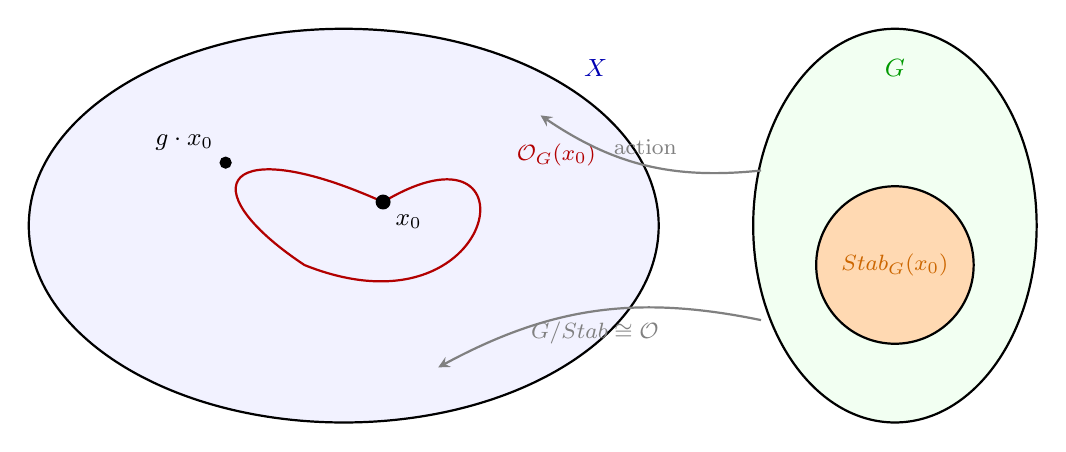
\begin{tikzpicture}[scale=1.0,>=stealth]
    \draw[thick, fill=blue!5] (0,0) ellipse (4 and 2.5);
    \node[font=\small\bfseries, blue!70!black] at (3.2, 2.0) {$X$};

    \draw[thick, red!70!black]
        (0.5,0.3) .. controls (2.5,1.5) and (2.0,-1.5) .. (-0.5,-0.5)
        .. controls (-2.0,0.5) and (-1.5,1.2) .. (0.5,0.3);
    \node[red!70!black, font=\footnotesize] at (2.7, 0.9) {$\mathcal{O}_G(x_0)$};

    \filldraw[black] (0.5, 0.3) circle (2.5pt);
    \node[font=\small, below right=1pt] at (0.5,0.3) {$x_0$};

    \filldraw[black] (-1.5, 0.8) circle (2pt);
    \node[font=\small, above left=1pt] at (-1.5,0.8) {$g\cdot x_0$};

    \draw[thick, fill=green!5] (7,0) ellipse (1.8 and 2.5);
    \node[font=\small\bfseries, green!60!black] at (7, 2.0) {$G$};

    \draw[thick, fill=orange!30] (7,-0.5) ellipse (1.0 and 1.0);
    \node[font=\footnotesize, orange!80!black, align=center] at (7,-0.5)
        {$\operatorname{Stab}_G(x_0)$};

    \draw[->, thick, gray] (5.3, 0.7) to[bend left=20]
        node[above, font=\footnotesize] {action} (2.5, 1.4);
    \draw[->, thick, gray] (5.3,-1.2) to[bend right=20]
        node[below, font=\footnotesize] {$G/\operatorname{Stab}\cong\mathcal{O}$} (1.2,-1.8);
\end{tikzpicture}
\caption{Group action, orbits and stabilisers. The relation between orbits and stabilisers is given by Lemma \ref{lem:orbit_stabilizer}.}
\label{fig:group_action_illustration}
\end{figure}

\section{Iteration: the starting point of every concept}

\begin{definition}[Iteration and discrete dynamical systems]\label{def:iteration}
Let $X$ be a non-empty set and $f:X\to X$ a map. The \textbf{iteration} of $f$ is defined by
\[
f^0=\operatorname{id}_X,\qquad f^{n+1}=f\circ f^n\quad(n\ge 0).
\]
The ordered pair $(X,f)$ is called a \textbf{discrete dynamical system}, and $f$ is called the \textbf{generator} or the \textbf{evolution map}. If $f$ is a bijection, negative iterates are defined by $f^{-n}=(f^{-1})^n$, so that iteration extends to the family with integer index $\{f^n\}_{n\in\mathbb{Z}}$.
\end{definition}

\begin{property}[The index law for iteration]\label{prop:iteration_law}
For all $m,n\ge 0$ (and $m,n\in\mathbb{Z}$ when $f$ is a bijection),
\[
f^{m+n}=f^m\circ f^n,\qquad f^{mn}=(f^m)^n.
\]
In particular, when $f$ is a bijection the map $n\mapsto f^n$ is a group homomorphism $(\mathbb{Z},+)\to\operatorname{Aut}(X)$, that is, iteration is equivalent to an action of $\mathbb{Z}$ on $X$.
\end{property}

\begin{proof}
Induct on $n$: $f^{m+0}=f^m=f^m\circ f^0$; suppose $f^{m+n}=f^m\circ f^n$, then
\[
f^{m+n+1}=f\circ f^{m+n}=f\circ f^m\circ f^n=f^{m+1}\circ f^n=f^m\circ f^{n+1}.
\]
The second identity follows from the first by induction on $n$. The case of negative indices follows from the definition of $(f^{-1})^n$ and the same induction. The homomorphism property is precisely the first identity.
\end{proof}

\begin{remark}[The primacy of iteration]\label{rem:iteration_primordial}
Iteration is logically prior to operations: addition, multiplication and exponentiation of the natural numbers are themselves generated recursively by `iteration of the successor map'. This chapter therefore takes iteration, rather than the group operation, as its starting point---a group is merely the algebraic structure that iteration self-organises into in the invertible case.
\end{remark}

\begin{definition}[Orbit]\label{def:orbit}
Let $(X,f)$ be a discrete dynamical system and $x_0\in X$. The \textbf{forward orbit} of $x_0$ is
\[
\mathcal{O}^+(x_0;f)=\{f^n(x_0)\mid n\ge 0\}.
\]
If $f$ is a bijection, the \textbf{(two-sided) orbit} of $x_0$ is
\[
\mathcal{O}(x_0;f)=\{f^n(x_0)\mid n\in\mathbb{Z}\}=\mathcal{O}_{\langle f\rangle}(x_0).
\]
\end{definition}

\begin{proposition}[Orbit partition]\label{prop:orbit_partition}
Let $f$ be a bijection. The relation
\[
x\sim y \iff \exists n\in\mathbb{Z},\ y=f^n(x)
\]
is an equivalence relation on $X$, and its equivalence classes are exactly the orbits. Hence the family of orbits forms a partition of $X$.
\end{proposition}

\begin{proof}
Reflexivity: $x=f^0(x)$. Symmetry: $y=f^n(x)\Rightarrow x=f^{-n}(y)$. Transitivity: $y=f^n(x),z=f^m(y)\Rightarrow z=f^{m+n}(x)$. The equivalence class is $[x]=\{f^n(x)\}=\mathcal{O}(x;f)$.
\end{proof}

\begin{definition}[Periodic points and eventually periodic points]\label{def:periodic_point}
Let $(X,f)$ be a discrete dynamical system and $x_0\in X$. If there exists an integer $m\ge 1$ such that
\[
f^m(x_0)=x_0,
\]
then $x_0$ is called a \textbf{periodic point}; the least positive integer $m_0$ satisfying the relation above is called the \textbf{least period} of $x_0$. If there exists $k\ge 0$ such that $f^k(x_0)$ is a periodic point, then $x_0$ is called an \textbf{eventually periodic point}.
\end{definition}

\begin{example}[A point that is eventually periodic but not periodic]\label{ex:eventually_periodic}
Let $X=\{0,1,2\}$, $f(0)=1$, $f(1)=2$, $f(2)=1$. Then $f^2(1)=1$, so $1$ and $2$ are periodic points; $f(0)=1$ and yet $0$ lies on no recurring orbit, so $0$ is an eventually periodic point but not a periodic point.
\end{example}

\begin{lemma}[Recurrence in invertible evolution]\label{lem:invertible_recurrence}
Let $f$ be a bijection and $x_0\in X$. If $x_0$ is an eventually periodic point, then $x_0$ is a periodic point.
\end{lemma}

\begin{proof}
Let $f^k(x_0)$ be a periodic point, with $f^m(f^k(x_0))=f^k(x_0)$ and $m\ge 1$. Applying $f^{-k}$ to both sides gives $f^m(x_0)=x_0$.
\end{proof}

\begin{figure}[htbp]
\centering
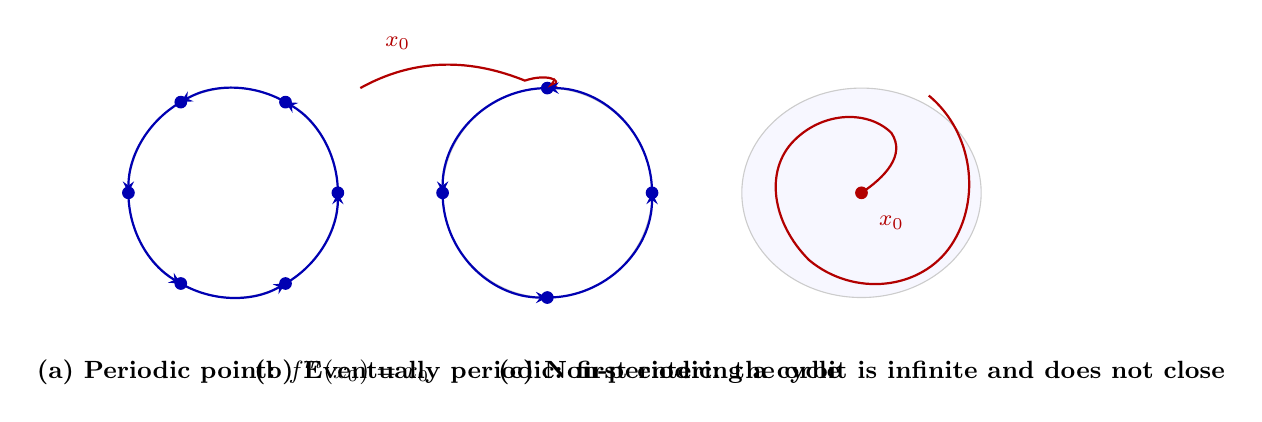
\begin{tikzpicture}[scale=0.95,>=stealth]

    \begin{scope}[shift={(-4.2,0)}]
        \draw[gray!40] (0,0) circle (1.4);
        \foreach \k in {0,1,...,5} {
            \filldraw[blue!70!black] ({60*\k}:1.4) circle (2.2pt);
        }
        \foreach \k in {0,1,...,5} {
            \draw[->, thick, blue!70!black] ({60*\k}:1.4) arc ({60*\k}:{60*(\k+1)}:1.4);
        }
        \node[font=\small\bfseries, below=2.0cm] at (0,0)
            {(a) Periodic point: $f^m(x_0)=x_0$};
    \end{scope}

    \begin{scope}[shift={(0,0)}]
        \draw[gray!40] (0,0) circle (1.4);
        \foreach \k in {0,1,...,3} {
            \filldraw[blue!70!black] ({90*\k}:1.4) circle (2.2pt);
        }
        \draw[->, thick, red!70!black]
            (-2.5,1.4) .. controls (-1.6,1.9) and (-0.8,1.7) .. (-0.3,1.5)
            .. controls (0.0,1.6) and (0.2,1.5) .. (0,1.4);
        \node[red!70!black, font=\footnotesize] at (-2.0,2.0) {$x_0$};
        \foreach \k in {0,1,...,3} {
            \draw[->, thick, blue!70!black] ({90*\k}:1.4) arc ({90*\k}:{90*(\k+1)}:1.4);
        }
        \node[font=\small\bfseries, below=2.0cm] at (0,0)
            {(b) Eventually periodic: first entering a cycle};
    \end{scope}

    \begin{scope}[shift={(4.2,0)}]
        \draw[gray!40, fill=blue!3] (0,0) ellipse (1.6 and 1.4);
        \draw[thick, red!70!black]
            (0,0) .. controls (0.3,0.2) and (0.6,0.5) .. (0.4,0.8)
            .. controls (0.1,1.1) and (-0.5,1.1) .. (-0.9,0.7)
            .. controls (-1.3,0.3) and (-1.2,-0.4) .. (-0.7,-0.9)
            .. controls (-0.1,-1.4) and (0.8,-1.3) .. (1.2,-0.7)
            .. controls (1.6,-0.1) and (1.5,0.8) .. (0.9,1.3);
        \filldraw[red!70!black] (0,0) circle (2.2pt);
        \node[red!70!black, font=\footnotesize] at (0.4,-0.4) {$x_0$};
        \node[font=\small\bfseries, below=2.0cm] at (0,0)
            {(c) Non-periodic: the orbit is infinite and does not close};
    \end{scope}

\end{tikzpicture}
\caption{The geometric shape of the three types of orbit: a periodic orbit closes; an eventually periodic orbit enters a closed cycle after finitely many steps; a non-periodic orbit extends indefinitely without closing.}
\label{fig:iteration_orbit_types}
\end{figure}

\section{Invariants and conservation}
\label{sec:invariants_conservation}

\begin{definition}[Invariant (conserved quantity)]\label{def:invariant}
Let $(X,f)$ be a discrete dynamical system. A map $Q:X\to Y$ is called an \textbf{invariant} of $f$ if
\[
Q\circ f=Q,\qquad\text{that is}\qquad Q(f(x))=Q(x),\quad\forall x\in X.
\]
When $Y=\mathbb{R}$, the map $Q$ is also called a \textbf{conserved quantity} or a \textbf{first integral}. If $Q$ is a constant map, it is called a \textbf{trivial invariant}; otherwise it is called a \textbf{non-trivial invariant}.
\end{definition}

\begin{proposition}[Orbit characterisation of invariants]\label{prop:invariant_orbit}
$Q$ is an invariant of $f$ if and only if $Q$ is constant on every forward orbit; when $f$ is a bijection, if and only if $Q$ is constant on every two-sided orbit.
\end{proposition}

\begin{proof}
If $Q\circ f=Q$, then induction on $n$ gives $Q\circ f^n=Q$, so $Q$ is identically $Q(x_0)$ on $\{f^n(x_0)\}$. Conversely, if $Q$ is constant on every forward orbit, then $Q(f(x))=Q(x)$ for every $x$. The bijective case is analogous.
\end{proof}

\begin{property}[Algebraic closure of invariants]\label{prop:invariant_algebra}
Let $Q_1,Q_2:X\to\mathbb{R}$ be $f$-conserved quantities and let $\varphi:\mathbb{R}^2\to\mathbb{R}$ be an arbitrary map. Then $x\mapsto\varphi(Q_1(x),Q_2(x))$ is again an $f$-conserved quantity. In particular, the set of all $f$-conserved quantities forms an $\mathbb{R}$-algebra.
\end{property}

\begin{proof}
Verify pointwise:
\[
\varphi(Q_1(f(x)),Q_2(f(x)))=\varphi(Q_1(x),Q_2(x)).
\]
\end{proof}

\begin{remark}[Triviality: the existence of a conserved quantity is not a condition]\label{rem:trivial_invariant}
A constant map is always an invariant of $f$, so `there exists a conserved quantity' holds for every system and imposes no constraint whatsoever. The statement with discriminating power is `there exists a \textbf{non-trivial} conserved quantity'. Listing `there exists a conserved quantity' as a necessary condition for periodicity is therefore an oversight: if `conservation' includes the trivial case, then the condition is always true and carries no information; if it is required to be non-trivial, then a periodic system need not satisfy it either.
\end{remark}

\begin{definition}[Conservation group]\label{def:conservation_group}
Let $Q:X\to Y$. The \textbf{conservation group} (equivariance group) of $Q$ is
\[
G_Q=\{g\in\operatorname{Aut}(X)\mid Q\circ g=Q\}.
\]
\end{definition}

\begin{property}[The conservation group is a group]\label{prop:conservation_group_is_group}
$G_Q\le\operatorname{Aut}(X)$.
\end{property}

\begin{proof}
$\operatorname{id}_X\in G_Q$. If $Q\circ g=Q$ and $Q\circ h=Q$, then $Q\circ(g\circ h)=Q$, and
\[
Q\circ g^{-1}=(Q\circ g)\circ g^{-1}=Q.
\]
Hence $G_Q$ is closed under composition and under taking inverses.
\end{proof}

\begin{proposition}[The evolution conserves its own invariants]\label{prop:f_in_GQ}
Let $f$ be a bijection and let $Q$ be an $f$-invariant. Then $\langle f\rangle\le G_Q$.
\end{proposition}

\begin{proof}
By Proposition \ref{prop:invariant_orbit}, $Q\circ f^n=Q$ for all $n\in\mathbb{Z}$. Hence $f^n\in G_Q$.
\end{proof}

\begin{remark}[Three sources of conserved quantities]\label{rem:conservation_source}
There are three routes to identifying a conserved quantity: \textbf{empirical observation}; \textbf{derivation from symmetry}; \textbf{mathematical structure} (a labelling function for the equivalence classes of orbits). All three produce functions that are constant on orbits.
\end{remark}

\begin{figure}[htbp]
\centering
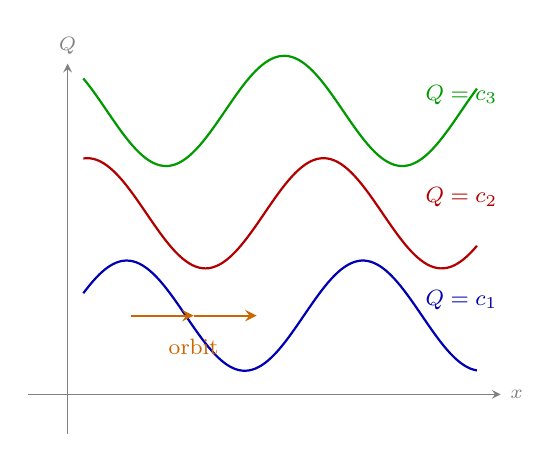
\begin{tikzpicture}[scale=1.0,>=stealth]
    \draw[->, gray] (-0.5,0) -- (5.5,0) node[right, font=\scriptsize] {$x$};
    \draw[->, gray] (0,-0.5) -- (0,4.2) node[above, font=\scriptsize] {$Q$};

    \draw[thick, blue!70!black, domain=0.2:5.2, samples=120]
        plot (\x, {1.0+0.7*sin(120*\x)});
    \draw[thick, red!70!black, domain=0.2:5.2, samples=120]
        plot (\x, {2.3+0.7*sin(120*\x+60)});
    \draw[thick, green!60!black, domain=0.2:5.2, samples=120]
        plot (\x, {3.6+0.7*sin(120*\x+120)});

    \node[blue!70!black, font=\footnotesize] at (5.0,1.2) {$Q=c_1$};
    \node[red!70!black, font=\footnotesize] at (5.0,2.5) {$Q=c_2$};
    \node[green!60!black, font=\footnotesize] at (5.0,3.8) {$Q=c_3$};

    \draw[->, thick, orange!80!black] (0.8,1.0) -- (1.6,1.0);
    \draw[->, thick, orange!80!black] (1.6,1.0) -- (2.4,1.0);
    \node[orange!80!black, font=\footnotesize] at (1.6,0.6) {orbit};
\end{tikzpicture}
\caption{The geometric picture of a conserved quantity $Q$: $Q$ is constant on every orbit, so orbits are confined within the level sets of $Q$. Distinct level sets give a stratification between the orbits.}
\label{fig:invariant_level_sets}
\end{figure}

\section{Symmetry}

\begin{definition}[Symmetry group of a dynamical system]\label{def:symmetry_group}
Let $(X,f)$ be a discrete dynamical system with $f$ a bijection. The \textbf{symmetry group} of $f$ is the centraliser of $f$ in $\operatorname{Aut}(X)$,
\[
\operatorname{Symmetry}(f)=\{g\in\operatorname{Aut}(X)\mid g\circ f=f\circ g\}
=C_{\operatorname{Aut}(X)}(f).
\]
\end{definition}

\begin{property}[The symmetry group is a group]\label{prop:symmetry_group_is_group}
$\operatorname{Symmetry}(f)\le\operatorname{Aut}(X)$, and $\langle f\rangle\le\operatorname{Symmetry}(f)$.
\end{property}

\begin{proof}
$\operatorname{id}_X$ commutes with $f$. If $g,h$ commute with $f$, then
\[
g\circ h\circ f=g\circ f\circ h=f\circ g\circ h,
\]
and
\[
g^{-1}\circ f=g^{-1}\circ f\circ g\circ g^{-1}
=g^{-1}\circ g\circ f\circ g^{-1}=f\circ g^{-1}.
\]
Hence $\operatorname{Symmetry}(f)$ is a subgroup. By Property \ref{prop:iteration_law}, $f^n\circ f=f^{n+1}=f\circ f^n$, so $\langle f\rangle\le\operatorname{Symmetry}(f)$.
\end{proof}

\begin{figure}[htbp]
\centering
\begin{tikzpicture}[>=stealth, node distance=3.2cm]
    \node (X1) {$X$};
    \node[right=of X1] (X2) {$X$};
    \node[below=2.2cm of X1] (X3) {$X$};
    \node[below=2.2cm of X2] (X4) {$X$};

    \draw[->, thick] (X1) -- node[above] {$f$} (X2);
    \draw[->, thick] (X1) -- node[left] {$g$} (X3);
    \draw[->, thick] (X2) -- node[right] {$g$} (X4);
    \draw[->, thick] (X3) -- node[below] {$f$} (X4);

    \node[font=\small, align=center] at (1.6,-1.2)
        {$g\in\operatorname{Symmetry}(f)$\\[2pt]
         if and only if $g\circ f=f\circ g$};
\end{tikzpicture}
\caption{The commutative-diagram definition of symmetry: evolving first and then transforming gives the same result as transforming first and then evolving. $\operatorname{Symmetry}(f)$ is precisely the group formed by all automorphisms $g$ that make this diagram commute.}
\label{fig:symmetry_commute}
\end{figure}

\begin{remark}[Why symmetry is defined via the centraliser]\label{rem:why_centraliser}
The mathematical meaning of `the laws of the system are the same before and after the transformation' is that evolving first and then transforming gives the same result as transforming first and then evolving, that is, the commutativity $g\circ f=f\circ g$. This definition does not depend on the existence of any conserved quantity, and hence makes `symmetry' and `conservation' two independent concepts.
\end{remark}

\begin{proposition}[Symmetry preserves orbits and least periods]\label{prop:symmetry_preserves_orbits}
Let $g\in\operatorname{Symmetry}(f)$ and $x_0\in X$. Then:
\begin{enumerate}[label=(\roman*)]
    \item $g$ maps $f$-orbits to $f$-orbits: $g(\mathcal{O}(x_0;f))=\mathcal{O}(g(x_0);f)$;
    \item $x_0$ is a periodic point if and only if $g(x_0)$ is a periodic point, and the two have the same least period.
\end{enumerate}
\end{proposition}

\begin{proof}
(i) From $g\circ f^n=f^n\circ g$ we get $g(f^n(x_0))=f^n(g(x_0))$; letting $n$ range over $\mathbb{Z}$ on both sides gives the result.

(ii) $f^m(g(x_0))=g(f^m(x_0))$, so $f^m(x_0)=x_0\iff f^m(g(x_0))=g(x_0)$. The least periods are therefore the same.
\end{proof}

\begin{definition}[Joint symmetry group of a system]\label{def:joint_symmetry}
Let $(X,f)$ be a discrete dynamical system and let $Q$ be an $f$-conserved quantity. The \textbf{joint symmetry group} of the triple $(X,f,Q)$ is
\[
\operatorname{Symmetry}(f,Q)=\operatorname{Symmetry}(f)\cap G_Q.
\]
\end{definition}

\begin{theorem}[Symmetry yields conservation (algebraic form)]\label{thm:symmetry_implies_conservation}
Let $f$ be a bijection, let $G\le\operatorname{Symmetry}(f)$, and suppose that every orbit of $G$ on $X$ is finite. Define the orbit-counting function
\[
Q_G:X\to\mathbb{N}\cup\{\infty\},\qquad Q_G(x)=|\mathcal{O}_G(x)|.
\]
Then $Q_G$ is an $f$-invariant. In particular, if the action of $G$ is non-trivial and not transitive, then $Q_G$ is a non-trivial $f$-conserved quantity.
\end{theorem}

\begin{proof}
For any $x\in X$, since $f$ commutes with every element of $G$,
\[
\mathcal{O}_G(f(x))=\{g\cdot f(x)\mid g\in G\}
=\{f(g\cdot x)\mid g\in G\}=f(\mathcal{O}_G(x)).
\]
Since $f$ is a bijection, its restriction to $\mathcal{O}_G(x)$ is a bijection onto $f(\mathcal{O}_G(x))$, so the two orbits have the same cardinality:
\[
Q_G(f(x))=Q_G(x).
\]
\end{proof}

\begin{remark}[Relation to Noether's theorem]\label{rem:noether}
What Theorem \ref{thm:symmetry_implies_conservation} proves is a kind of \textbf{orbit-counting construction of invariants}, not Noether's theorem. It is merely the purely algebraic version of `symmetry $\Rightarrow$ conservation'. The stronger Noether theorem in physics requires a Lagrangian variational structure and the language of Lie algebras, and lies outside the framework of this chapter.
\end{remark}

\begin{proposition}[Conservation does not imply symmetry]\label{prop:conservation_not_symmetry}
There exists a system $(X,f,Q)$ in which $Q$ is a non-trivial $f$-conserved quantity, yet the joint symmetry group $\operatorname{Symmetry}(f,Q)$ is trivial.
\end{proposition}

\begin{proof}
Take $X=\mathbb{R}$, $f=\operatorname{id}_{\mathbb{R}}$ and $Q(x)=x^3+x$. Here every function is an $f$-invariant, so $Q$ is conserved and non-trivial. Note that $Q'(x)=3x^2+1>0$, so $Q$ is strictly increasing and hence injective. If $g\in G_Q$, then $Q(g(x))=Q(x)$ for all $x$, and the injectivity of $Q$ gives $g(x)=x$, that is, $G_Q=\{\operatorname{id}\}$. Hence
\[
\operatorname{Symmetry}(f,Q)=\operatorname{Symmetry}(f)\cap G_Q=\{\operatorname{id}\}.
\]
\end{proof}

\begin{remark}[The reflection trap in constructing counterexamples]\label{rem:counterexample_fix}
In constructing a counterexample of the form `conserved but with trivial symmetry', the choice $Q(x)=x^2$ does not work: the reflection $x\mapsto -x$ satisfies $(-x)^2=x^2$, so $G_Q\supseteq\{\operatorname{id},x\mapsto -x\}\cong C_2$. A conserved quantity of injective type must be used.
\end{remark}

\begin{corollary}[The logical hierarchy of conservation and symmetry]\label{cor:conservation_symmetry_hierarchy}
\begin{enumerate}[label=(\roman*)]
    \item symmetry $\Rightarrow$ conservation (Theorem \ref{thm:symmetry_implies_conservation}, requiring finite $G$-orbits);
    \item conservation $\nRightarrow$ symmetry (Proposition \ref{prop:conservation_not_symmetry});
    \item hence symmetry is a strictly stronger concept than conservation.
\end{enumerate}
\end{corollary}

\section{Finite-order actions}

\begin{definition}[Order of a map]\label{def:map_order}
Let $f:X\to X$. If there exists a least positive integer $m$ such that $f^m=\operatorname{id}_X$, then $f$ is called a \textbf{finite-order action} and $m$ is its \textbf{order}, written $\operatorname{ord}(f)=m$; otherwise we write $\operatorname{ord}(f)=\infty$. When $f$ is a bijection, this is equivalent to the order of the cyclic subgroup $\langle f\rangle\le\operatorname{Aut}(X)$.
\end{definition}

\begin{lemma}[Finite order implies invertibility]\label{lem:finite_order_bijective}
If $\operatorname{ord}(f)=m<\infty$, then $f$ must be a bijection, and $f^{-1}=f^{m-1}$.
\end{lemma}

\begin{proof}
$f\circ f^{m-1}=f^m=\operatorname{id}_X=f^{m-1}\circ f$, so $f^{m-1}$ is a two-sided inverse of $f$.
\end{proof}

\begin{lemma}[Pointwise closure and uniform closure]\label{lem:pointwise_vs_uniform}
Let $f$ be a bijection. Distinguish the following two concepts:
\begin{enumerate}[label=(\roman*)]
    \item \textbf{pointwise closure}: every $x\in X$ is a periodic point (the least periods $m_x$ of different points may differ);
    \item \textbf{uniform closure}: $\operatorname{ord}(f)<\infty$ (there exists a uniform $m$ with $f^m=\operatorname{id}_X$).
\end{enumerate}
Then (ii) $\Rightarrow$ (i), and in that case every $m_x$ divides $\operatorname{ord}(f)$; but (i) $\nRightarrow$ (ii).
\end{lemma}

\begin{proof}
(ii) $\Rightarrow$ (i): $f^m(x)=x$ for all $x$. Let $m_x$ be the least period of $x$ and perform division with remainder $m=qm_x+r$, $0\le r<m_x$; then
\[
f^r(x)=f^{m-qm_x}(x)=f^m(x)=x,
\]
and the minimality of $m_x$ gives $r=0$, that is, $m_x\mid m$.

(i) $\nRightarrow$ (ii): Take $X=\bigsqcup_{n\ge 1}\mathbb{Z}/n\mathbb{Z}$, and on the $n$-th component let $f$ be the map `add $1$', $x\mapsto x+1\pmod n$. Every point belongs to some component and has least period $n$, so (i) holds. But for any $m\ge 1$, on the $(m+1)$-th component $f^m(0)=m\not\equiv 0\pmod{m+1}$, so $f^m\neq\operatorname{id}_X$ and $\operatorname{ord}(f)=\infty$.
\end{proof}

\begin{figure}[htbp]
\centering
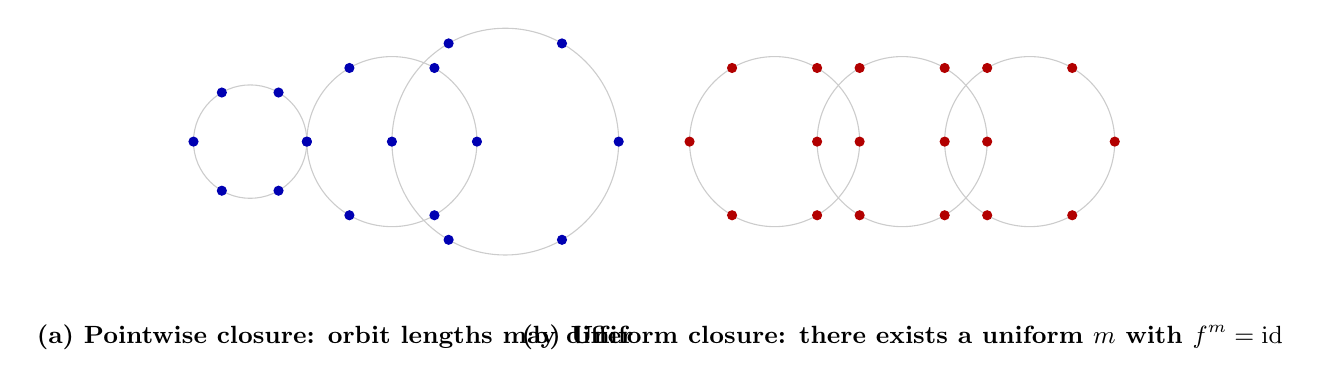
\begin{tikzpicture}[scale=0.9,>=stealth]

    \begin{scope}[shift={(-4,0)}]
        \foreach \r/\x in {0.8/-1.2, 1.2/0.8, 1.6/2.4} {
            \draw[gray!40] (\x,0) circle (\r);
            \foreach \k in {0,1,...,5} {
                \filldraw[blue!70!black] ({\x+\r*cos(60*\k)},{\r*sin(60*\k)}) circle (1.8pt);
            }
        }
        \node[font=\small\bfseries, below=2.2cm] at (0,0)
            {(a) Pointwise closure: orbit lengths may differ};
    \end{scope}

    \begin{scope}[shift={(4,0)}]
        \foreach \x in {-1.8,0,1.8} {
            \draw[gray!40] (\x,0) circle (1.2);
            \foreach \k in {0,1,...,5} {
                \filldraw[red!70!black] ({\x+1.2*cos(60*\k)},{1.2*sin(60*\k)}) circle (1.8pt);
            }
        }
        \node[font=\small\bfseries, below=2.2cm] at (0,0)
            {(b) Uniform closure: there exists a uniform $m$ with $f^m=\mathrm{id}$};
    \end{scope}

\end{tikzpicture}
\caption{Pointwise closure requires only that each point returns to itself, and the periods may differ; uniform closure requires a uniform $m$ such that all points return simultaneously. Passing from the former to the latter requires `periods uniformly bounded' or a `finite least common multiple'.}
\label{fig:pointwise_vs_uniform}
\end{figure}

\begin{theorem}[Orbit characterisation of finite order]\label{thm:finite_order_orbit}
Let $f$ be a bijection. The following conditions are equivalent:
\begin{enumerate}[label=(\roman*)]
    \item $\operatorname{ord}(f)=m<\infty$;
    \item $f$ is pointwise closed, and the least common multiple of all the least periods $\{m_x\}$ is finite;
    \item $f$ is pointwise closed, and the orbit lengths are uniformly bounded.
\end{enumerate}
When the equivalence holds,
\[
\operatorname{ord}(f)=\operatorname{lcm}\{m_x\mid x\in X\}.
\]
\end{theorem}

\begin{proof}
(i) $\Rightarrow$ (ii): By Lemma \ref{lem:pointwise_vs_uniform}, every $m_x\mid m$, so $\operatorname{lcm}\{m_x\}\mid m$ is finite.

(ii) $\Rightarrow$ (i): Let $M=\operatorname{lcm}\{m_x\}<\infty$. For any $x$, $m_x\mid M$, so $f^M(x)=x$, that is, $f^M=\operatorname{id}_X$. Also every $m_x\mid\operatorname{ord}(f)$, so $M\mid\operatorname{ord}(f)$, and the two are equal.

(ii) $\Rightarrow$ (iii): $m_x\le M$, so the periods are uniformly bounded.

(iii) $\Rightarrow$ (ii): If $m_x\le N$ for all $x$, then $\operatorname{lcm}\{m_x\}\mid\operatorname{lcm}(1,2,\dots,N)$, which is finite.
\end{proof}

\begin{remark}[A point on rigour]\label{rem:finite_order_caution}
In passing from `each orbit closes on its own' to `finite-order action', the additional condition of \textbf{uniformly bounded periods} (or a finite least common multiple) must be imposed. If the `closure group' is defined as the subgroup generated by elements of finite order, $G_{\mathrm{cl}}=\langle g\in G:\operatorname{ord}(g)<\infty\rangle$, it guarantees only that each generator has finite pointwise order, and does not automatically give uniform closure of the whole action.
\end{remark}

\section{Closed orbits and periodicity}

\begin{definition}[Closed orbit]\label{def:closed_orbit}
Let $(X,f)$ be a discrete dynamical system. An orbit $\mathcal{O}(x_0;f)$ (or a forward orbit $\mathcal{O}^+(x_0;f)$) is called \textbf{closed} if it is a finite set.
\end{definition}

\begin{theorem}[Criterion for closed orbits]\label{thm:closed_orbit_criterion}
Let $f$ be a bijection and $x_0\in X$. The following conditions are equivalent:
\begin{enumerate}[label=(\roman*)]
    \item the orbit $\mathcal{O}(x_0;f)$ is closed;
    \item $x_0$ is a periodic point;
    \item the stabiliser $\operatorname{Stab}_{\langle f\rangle}(x_0)$ has finite index in $\langle f\rangle$.
\end{enumerate}
When the equivalence holds,
\[
|\mathcal{O}(x_0;f)|=m_0=\text{the least period of $x_0$},
\qquad
\operatorname{Stab}_{\langle f\rangle}(x_0)=\langle f^{m_0}\rangle,
\]
and the restriction of $f$ to the orbit is an $m_0$-cycle permutation.
\end{theorem}

\begin{proof}
(i) $\Rightarrow$ (ii): If the orbit is finite, then the infinite sequence $x_0,f(x_0),f^2(x_0),\dots$ must contain a repetition: there exist $i<j$ with $f^i(x_0)=f^j(x_0)$. Applying $f^{-i}$ to both sides gives $f^{j-i}(x_0)=x_0$, so $x_0$ is a periodic point.

(ii) $\Rightarrow$ (i) and the structure of the orbit: Let $f^{m_0}(x_0)=x_0$ with $m_0$ least. For any $n\in\mathbb{Z}$, division with remainder $n=qm_0+r$ gives $f^n(x_0)=f^r(x_0)$, so
\[
\mathcal{O}(x_0;f)=\{x_0,f(x_0),\dots,f^{m_0-1}(x_0)\}.
\]
These $m_0$ points are pairwise distinct: if $f^r(x_0)=f^s(x_0)$ with $0\le r<s<m_0$, then $f^{s-r}(x_0)=x_0$, contradicting the minimality of $m_0$. Hence the orbit contains exactly $m_0$ points. Also $f(f^{m_0-1}(x_0))=x_0$, so $f$ permutes the orbit cyclically.

(ii) $\iff$ (iii): $f^n\in\operatorname{Stab}(x_0)\iff f^n(x_0)=x_0\iff m_0\mid n$, so the stabiliser is exactly $\langle f^{m_0}\rangle$, with index $m_0$.
\end{proof}

\begin{figure}[htbp]
\centering
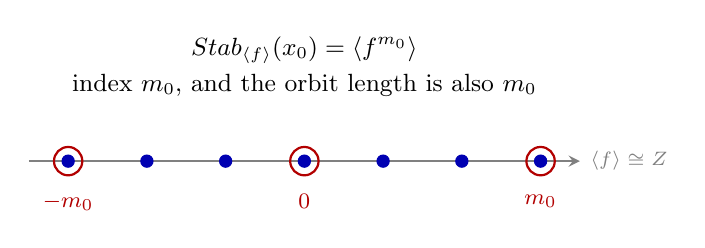
\begin{tikzpicture}[scale=1.0,>=stealth]
    \draw[->, thick, gray] (-3.5,0) -- (3.5,0) node[right, font=\scriptsize] {$\langle f\rangle\cong\mathbb Z$};

    \foreach \x in {-3,...,3} {
        \draw[gray] (\x,0.08) -- (\x,-0.08);
    }

    \foreach \x in {-3,-2,-1,0,1,2,3} {
        \filldraw[blue!70!black] (\x,0) circle (2.2pt);
    }

    \foreach \x in {-3,0,3} {
        \draw[red!70!black, thick] (\x,0) circle (0.18);
    }

    \node[red!70!black, font=\footnotesize, below] at (-3,-0.3) {$-m_0$};
    \node[red!70!black, font=\footnotesize, below] at (0,-0.3) {$0$};
    \node[red!70!black, font=\footnotesize, below] at (3,-0.3) {$m_0$};

    \node[font=\small, align=center] at (0,1.2)
        {$\operatorname{Stab}_{\langle f\rangle}(x_0)=\langle f^{m_0}\rangle$\\[2pt]
         index $m_0$, and the orbit length is also $m_0$};
\end{tikzpicture}
\caption{On a closed orbit the stabiliser is exactly $\langle f^{m_0}\rangle$, and its index in $\langle f\rangle$ equals the orbit length $m_0$.}
\label{fig:closed_orbit_stabilizer}
\end{figure}

\begin{corollary}[Periodic structure of closed orbits]\label{cor:closed_orbit_structure}
The dynamical system on a closed orbit, $(\mathcal{O}(x_0;f),f|_{\mathcal{O}})$, is isomorphic to the action of the cyclic group $C_{m_0}$ by translation on itself ($k\mapsto k+1\bmod m_0$).
\end{corollary}

\begin{proof}
By Theorem \ref{thm:closed_orbit_criterion}, the orbit is exactly $\{x_0,\dots,f^{m_0-1}(x_0)\}$ and $f$ cycles on it. The map $f^k(x_0)\mapsto k\bmod m_0$ is a bijection of sets, and conjugates $f|_{\mathcal{O}}$ to the map `add $1$' on $\mathbb{Z}/m_0\mathbb{Z}$.
\end{proof}

\begin{definition}[Strict periodicity]\label{def:strict_period}
A discrete dynamical system $(X,f)$ is said to have a \textbf{strict period} at $x_0$ if $x_0$ is a periodic point; its least period $m_0$ is called the \textbf{period} of the system at $x_0$. If every point is a periodic point, the system is called a \textbf{periodic system}; if moreover $\operatorname{ord}(f)=m<\infty$, the system is called a \textbf{uniformly periodic system}, and $m$ is its \textbf{uniform period}.
\end{definition}

\begin{remark}[The place of quasiperiodicity]\label{rem:quasi_period}
`Quasiperiodicity' (for instance an irrational rotation of the circle: the orbit does not close but is dense) is essentially a topological concept. Within a purely algebraic framework one can only assert that $\operatorname{ord}(f)=\infty$. This chapter distinguishes only: trivial periodicity ($m_0=1$, a fixed point), strict periodicity ($m_0\ge 2$) and aperiodicity (an infinite orbit).
\end{remark}

\begin{proposition}[Periodicity yields symmetry]\label{prop:period_implies_symmetry}
Let $f$ be a bijection with $\operatorname{ord}(f)=m<\infty$. Then the evolution group $\langle f\rangle\cong C_m$ is a non-trivial (when $m\ge 2$) finite subgroup of $\operatorname{Symmetry}(f)$.
\end{proposition}

\begin{proof}
By Property \ref{prop:symmetry_group_is_group}, $\langle f\rangle\le\operatorname{Symmetry}(f)$; by Definition \ref{def:map_order}, $|\langle f\rangle|=m$.
\end{proof}

\begin{theorem}[Periodicity does not imply non-trivial conservation]\label{thm:period_not_imply_conservation}
There exists a uniformly periodic system all of whose $f$-conserved quantities are trivial (constant).
\end{theorem}

\begin{proof}
Take $X=\mathbb{Z}/m\mathbb{Z}$ ($m\ge 2$) and $f(x)=x+1\pmod m$. Then $f^m=\operatorname{id}_X$ with $m$ least, so the system is uniformly periodic. Let $Q:X\to Y$ be an arbitrary $f$-invariant. By Proposition \ref{prop:invariant_orbit}, $Q$ is constant on every orbit; but $f$ has only one orbit on $X$, so $Q$ is constant on the whole of $X$.
\end{proof}

\begin{remark}[The hierarchical difference between periodicity and conservation]\label{rem:gap_diagnosis}
The stronger the transitivity of the orbits, the fewer the invariants. A periodic orbit is precisely the `most transitive' structure---the whole orbit is a single cycle, and any conserved quantity must take the same value everywhere. Hence `periodicity $\Rightarrow$ conservation' fails in general. A conserved quantity describes the stratification \textbf{between orbits}, not the cycle within an orbit.
\end{remark}

\begin{corollary}[Logical diagram of period, symmetry and conservation]\label{cor:true_logic}
\begin{enumerate}[label=(\roman*)]
    \item finite order $\Rightarrow$ uniform periodicity $\Rightarrow$ pointwise periodicity $\iff$ pointwise closed orbits;
    \item periodicity $\Rightarrow$ symmetry, but periodicity $\nRightarrow$ conservation;
    \item symmetry $\Rightarrow$ conservation, but conservation $\nRightarrow$ symmetry;
    \item the conjunction of symmetry and conservation still $\nRightarrow$ periodicity: take $X=\mathbb{R}$, $f(x)=x+1$, $Q(x)=\sin(2\pi x)$. Then $Q\circ f=Q$ and $\langle f\rangle\cong\mathbb{Z}$ is non-trivial with $\langle f\rangle\le\operatorname{Symmetry}(f,Q)$; but $\operatorname{ord}(f)=\infty$.
\end{enumerate}
\end{corollary}

\begin{proof}
(i) By Definition \ref{def:strict_period}, Theorem \ref{thm:closed_orbit_criterion} and Lemma \ref{lem:pointwise_vs_uniform}. (ii) Proposition \ref{prop:period_implies_symmetry} and Theorem \ref{thm:period_not_imply_conservation}. (iii) Theorem \ref{thm:symmetry_implies_conservation} and Proposition \ref{prop:conservation_not_symmetry}. (iv) Verify item by item: $Q(f(x))=\sin(2\pi(x+1))=\sin(2\pi x)=Q(x)$; $f$ commutes with itself and preserves $Q$; $f^n(x)=x+n\neq x$, so there are no periodic points.
\end{proof}

\begin{remark}[The logical structure of the main chain]\label{rem:chain_verdict}
In the chain `conservation $\to$ symmetry $\to$ closed orbit $\to$ period': the first step has the opposite direction (it is really symmetry $\Rightarrow$ conservation), the second step does not hold (symmetry $+$ conservation $\nRightarrow$ finite order), and the third step holds and is reversible (closed orbit $\iff$ pointwise periodicity). Within the framework of this chapter the unconditional sufficient chain is
\[
\text{finite-order action}\Longrightarrow\text{(uniform) closed orbit}\Longrightarrow\text{strict period}.
\]
The proper role of conservation and symmetry here is this: symmetry restricts the possible forms of the evolution, and conservation confines the orbits to low-dimensional level sets---the two are auxiliary tools for \textbf{discovering and proving} that some generator has finite order, not an indispensable link in the chain of logic.
\end{remark}

\section{Function characteristics of the three elementary transformations}
\label{sec:function_features_transformations}

This section characterises the three elementary transformations---translation, scaling and rotation---from the point of view of functional equations.

\begin{definition}[Translation-symmetric and translation-covariant functions]\label{def:translation_symmetric_function}
Let $f:\mathbb{R}\to Y$. If there exists $a\neq 0$ such that
\[
f(x+a)=f(x),\qquad \forall x\in\mathbb{R},
\]
then $f$ is called a \textbf{translation-symmetric function} and $a$ is called a \textbf{translation period}. If there exists $\lambda\in\mathbb{C}$ with $|\lambda|=1$ such that
\[
f(x+a)=\lambda f(x),\qquad \forall x,
\]
then $f$ is called a \textbf{translation-covariant function} and $\lambda$ is called the \textbf{translation characteristic factor}.
\end{definition}

\begin{definition}[Scaling-symmetric and homogeneous functions]\label{def:scaling_symmetric_function}
Let $f:\mathbb{R}^+\to Y$. If there exists $q>0$, $q\neq 1$, such that
\[
f(qx)=f(x),\qquad \forall x>0,
\]
then $f$ is called a \textbf{scaling-symmetric function} and $q$ is called a \textbf{scaling period}. If there exists $s\in\mathbb{R}$ such that
\[
f(qx)=q^s f(x),\qquad \forall x>0,
\]
then $f$ is called a \textbf{homogeneous function} and $s$ is called the \textbf{homogeneity exponent}.
\end{definition}

\begin{definition}[Rotation-symmetric and rotation-covariant functions]\label{def:rotation_symmetric_function}
Let $f:\mathbb{C}^\times\to Y$. If there exists $\theta\in\mathbb{R}$ such that
\[
f(e^{i\theta}z)=f(z),\qquad \forall z\neq 0,
\]
then $f$ is called a \textbf{rotation-symmetric function} and $\theta$ is called a \textbf{rotation period}. If there exists $m\in\mathbb{Z}$ such that
\[
f(e^{i\theta}z)=e^{im\theta}f(z),\qquad \forall z\neq 0,
\]
then $f$ is called a \textbf{rotation-covariant function} and $m$ is called the \textbf{weight}.
\end{definition}

\begin{definition}[Group of period transformations]\label{def:period_group}
Let $G$ be a transformation group and $f:X\to Y$. The \textbf{group of period transformations} of $f$ is
\[
\operatorname{Group}_{\mathrm{period},G}(f)
=\{g\in G\mid f(g\cdot x)=f(x),\ \forall x\in X\}.
\]
\end{definition}

\begin{proposition}[Translation symmetry and antiperiodicity]\label{prop:translation_antiperiod}
Let $f:\mathbb{R}\to Y$ and $a\neq 0$.
\begin{enumerate}[label=(\roman*)]
    \item If $f(x+a)=f(x)$, then every element of $a\mathbb{Z}$ is a translation period of $f$.
    \item If $f(x+a)=-f(x)$, then $f(x+2a)=f(x)$.
    \item More generally, if $f(x+a)+f(x)=c$ is constant, then $f(x+2a)=f(x)$ still holds.
\end{enumerate}
\end{proposition}

\begin{proof}
(i) Iterating $f(x+a)=f(x)$ repeatedly gives $f(x+na)=f(x)$.

(ii) $f(x+2a)=f((x+a)+a)=-f(x+a)=f(x)$.

(iii) Subtracting $f(x+a)+f(x)=c$ from $f(x+2a)+f(x+a)=c$ gives $f(x+2a)=f(x)$.
\end{proof}

\begin{proposition}[Scaling symmetry and logarithmic translation]\label{prop:scaling_log_translation}
Let $f:\mathbb{R}^+\to Y$, $q>0$, $q\neq 1$. Put
\[
g(t):=f(e^t),\qquad t\in\mathbb{R}.
\]
Then
\[
f(qx)=f(x)\quad\Longleftrightarrow\quad g(t+\ln q)=g(t).
\]
Hence a scaling-symmetric function is equivalent to a translation-symmetric function in logarithmic coordinates. Conversely, if $q=e^\alpha$ with $\alpha\neq 0$ and $g(t+\alpha)=g(t)$, then $f(qx)=f(x)$.
\end{proposition}

\begin{proof}
Substituting $x=e^t$ gives
\[
f(qe^t)=f(e^{t+\ln q})=g(t+\ln q).
\]
Hence $f(qx)=f(x)$ is equivalent to $g(t+\ln q)=g(t)$. Conversely, if $q=e^\alpha$ and $g(t+\alpha)=g(t)$, then for $x=e^t>0$,
\[
f(qx)=f(e^\alpha e^t)=f(e^{t+\alpha})=g(t+\alpha)=g(t)=f(x).
\]
\end{proof}

\begin{proposition}[Rotation symmetry and the order of roots of unity]\label{prop:rotation_unit_root_order}
Let $f:\mathbb{C}^\times\to Y$, $a\in\mathbb{N}^+$ and $q\in\mathbb{Z}$. If
\[
f(e^{2\pi i q/a}z)=f(z),\qquad \forall z\neq 0,
\]
then
\[
C_{a/\gcd(a,q)}\le \operatorname{Group}_{\mathrm{period},U(1)}(f),
\]
where for $q=0$ we adopt the convention $a/\gcd(a,0)=1$.
\end{proposition}

\begin{proof}
The order of the element $e^{2\pi i q/a}$ is
\[
\operatorname{ord}\!\left(e^{2\pi i q/a}\right)=\frac{a}{\gcd(a,q)}.
\]
Hence the cyclic group it generates is $C_{a/\gcd(a,q)}$, and every element of this group leaves $f$ invariant.
\end{proof}

\begin{example}[Translation symmetry]\label{ex:translation_symmetric}
$f(x)=\sin(2\pi x/a)$ satisfies $f(x+a)=f(x)$, and its least positive period is $a$.
\end{example}

\begin{example}[Antiperiodicity]\label{ex:antiperiod}
$f(x)=(-1)^{\lfloor x/a\rfloor}$ satisfies $f(x+a)=-f(x)$, so $f(x+2a)=f(x)$ and the period is doubled to $2a$.
\end{example}

\begin{example}[Scaling symmetry]\label{ex:scaling_symmetric}
$f(x)=\sin(2\pi\log_q x)$, $x>0$, satisfies $f(qx)=f(x)$.
\end{example}

\begin{example}[Rotation symmetry]\label{ex:rotation_symmetric}
$f(z)=z^n$ satisfies
\[
f(e^{2\pi i/n}z)=e^{2\pi i}z^n=z^n=f(z),
\]
so the rotation group with periodic orbits contains $C_n$.
\end{example}

\begin{remark}[Function characteristics of the three transformations compared]\label{rem:three_transformations_function_features}
\begin{center}
\begin{tabular}{@{}p{2.2cm}p{5.2cm}p{5.0cm}@{}}
\toprule
Transformation & Functional equation & Characteristic \\
\midrule
Translation & $f(x+a)=f(x)$ & translation-invariant, with period $a$ \\
Translation & $f(x+a)=-f(x)$ & antiperiodic, with period doubled to $2a$ \\
Scaling & $f(qx)=f(x)$ & scaling-invariant, a translation period in logarithmic coordinates \\
Rotation & $f(e^{i\theta}z)=f(z)$ & rotation-invariant, the group with periodic orbits being determined by the order of roots of unity \\
\bottomrule
\end{tabular}
\end{center}
\end{remark}

\begin{remark}[Interface with the extensions of number systems]\label{rem:function_features_number_systems}
The three functional equations given in this section have, respectively, three algebraic structures as their background:
\[
\text{translation: the additive group }(\mathbb{R},+),\qquad
\text{scaling: the multiplicative group }(\mathbb{R}^+,\times),\qquad
\text{rotation: the circle group }U(1).
\]
The minimal algebraic realisations of these three groups within the number systems correspond to the main line of the extension of number systems in the next chapter:
\begin{enumerate}[label=(\roman*)]
    \item \textbf{Translation} requires the freedom to add and subtract the period $a$, so at least the additive group of the integers $\mathbb{Z}$ is needed.
    \item \textbf{Scaling} requires the freedom to multiply and divide by the period $q$, so at least the multiplicative group of the positive rationals $\mathbb{Q}^+$ is needed.
    \item \textbf{Rotation} requires unit complex numbers $e^{i\theta}$, so at least the unit circle group $U(1)$ of the complex numbers $\mathbb{C}$ is needed.
    \item \textbf{Three-dimensional rotation} requires a more general non-commutative rotation group. Its double cover is the unit sphere group $S^3\cong SU(2)$ of the quaternions $\mathbb{H}$, and the rotation group itself is $SO(3)\cong SU(2)/\{\pm I\}$.
\end{enumerate}
Thus each step in the extension of the number systems makes a new class of periodic transformations decidable.
\end{remark}

\begin{remark}[Connection with the group action framework]\label{rem:function_features_group_action}
The functional equations given in this section are all concrete manifestations of group actions on function spaces. The group with periodic orbits $\operatorname{Group}_{\mathrm{period},G}(f)$ is precisely the set of transformations for which the corresponding functional equation holds. Hence
\[
\text{the transformation }g\text{ is a period of }f
\iff
f(g\cdot x)=f(x),\quad \forall x.
\]
\end{remark}

\begin{remark}[Boundaries of domain and order]\label{rem:function_features_boundary}
\begin{enumerate}[label=(\roman*)]
    \item A scaling period is usually defined for $x>0$ or $x\neq 0$, because the multiplicative action of $q>0$ is most natural on $\mathbb{R}^+$.
    \item For a rotation period, if $a\notin\mathbb{N}^+$ then $e^{2\pi i/a}$ need not be a root of unity, and its order may be infinite; the statement `the rotation period is $a$' therefore holds only when $a$ is a positive integer and a primitive root of unity is taken.
    \item Antiperiodicity $f(x+a)+f(x)=0$ is not itself a period, but it implies the period $2a$.
\end{enumerate}
\end{remark}

\begin{figure}[htbp]
\centering
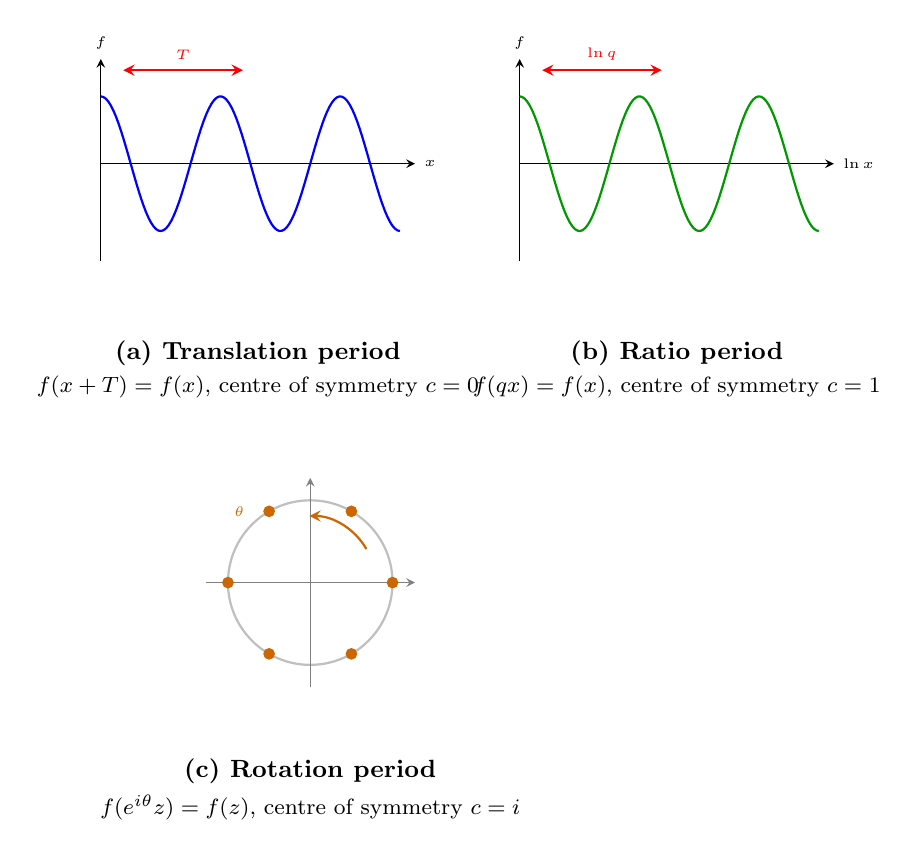
\begin{tikzpicture}[>=stealth, scale=0.95,
    box/.style={draw, rounded corners=2pt, align=center, font=\small\bfseries, inner sep=4pt}]

    \begin{scope}[shift={(0,0)}]
        \draw[->] (0,0) -- (4.2,0) node[right, font=\tiny] {$x$};
        \draw[->] (0,-1.3) -- (0,1.4) node[above, font=\tiny] {$f$};
        \draw[thick, blue, domain=0:4, samples=120]
            plot (\x, {0.9*cos(360*\x/1.6)});
        \draw[<->, thick, red] (0.3,1.25) -- (1.9,1.25)
            node[midway, above, font=\tiny] {$T$};
        \node[font=\small\bfseries, below=0.6cm] at (2.1,-1.6)
            {(a) Translation period};
        \node[font=\footnotesize, below=1.05cm] at (2.1,-1.6)
            {$f(x+T)=f(x)$, centre of symmetry $c=0$};
    \end{scope}

    \begin{scope}[shift={(5.6,0)}]
        \draw[->] (0,0) -- (4.2,0)
            node[right, font=\tiny] {$\ln x$};
        \draw[->] (0,-1.3) -- (0,1.4) node[above, font=\tiny] {$f$};
        \draw[thick, green!60!black, domain=0:4, samples=120]
            plot (\x, {0.9*cos(360*\x/1.6)});
        \draw[<->, thick, red] (0.3,1.25) -- (1.9,1.25)
            node[midway, above, font=\tiny] {$\ln q$};
        \node[font=\small\bfseries, below=0.6cm] at (2.1,-1.6)
            {(b) Ratio period};
        \node[font=\footnotesize, below=1.05cm] at (2.1,-1.6)
            {$f(qx)=f(x)$, centre of symmetry $c=1$};
    \end{scope}

    \begin{scope}[shift={(2.8,-5.6)}]
        \draw[thick, gray!50] (0,0) circle (1.1);
        \draw[->, gray] (-1.4,0) -- (1.4,0);
        \draw[->, gray] (0,-1.4) -- (0,1.4);
        \foreach \k in {0,1,...,5} {
            \filldraw[orange!80!black]
                ({\k*60}:1.1) circle (2pt);
        }
        \draw[->, thick, orange!80!black] (0.75,0.45) arc (30:90:0.88);
        \node[font=\tiny, orange!80!black] at (-0.95,0.95) {$\theta$};
        \node[font=\small\bfseries, below=0.6cm] at (0,-1.6)
            {(c) Rotation period};
        \node[font=\footnotesize, below=1.05cm] at (0,-1.6)
            {$f(e^{i\theta}z)=f(z)$, centre of symmetry $c=i$};
    \end{scope}
\end{tikzpicture}
\caption{The three fundamental types of periodic function. They are governed respectively by the centres of symmetry $0$, $1$ and $i$. Note that the ratio period in (b) degenerates to a translation period in logarithmic coordinates.}
\label{fig:three_types_periodicity}
\end{figure}

\section{Completeness of the three elementary transformations: classification of one-parameter families of conformal transformations}
\label{sec:completeness_three_transformations}

The preceding sections of this chapter introduced translation, scaling and rotation as the three elementary transformations and gave their functional equations one by one. This section answers a stronger question: \textbf{why exactly these three?} Below, within the explicit framework of `one-parameter families of conformal transformations on the complex plane', we prove that the three constitute a \textbf{complete and mutually exclusive} set of generating primitives. It should be declared in advance that the scope of the conclusions of this section is precisely this framework; the corresponding assertion for general continuous transformation groups is not among the claims of this book (see `what this book does not claim' in the introduction, and Remark \ref{rem:completeness_boundary} at the end of this section).

\subsection{One-parameter families of transformations and infinitesimal generators}

\begin{definition}[One-parameter families of transformations]\label{def:one_parameter_family}
Let $\Omega\subseteq\hat{\mathbb C}=\mathbb C\cup\{\infty\}$ be an open set. A family of maps $\{\varphi_t\}_{t\in\mathbb R}$, $\varphi_t:\Omega\to\Omega$, is called a \textbf{one-parameter family of transformations} if
\begin{enumerate}[label=(\roman*)]
    \item $\varphi_0=\operatorname{id}$;
    \item $\varphi_{s+t}=\varphi_s\circ\varphi_t$ for all $s,t\in\mathbb R$ (that is, $t\mapsto\varphi_t$ is a group homomorphism);
    \item $(t,z)\mapsto\varphi_t(z)$ is smooth in $t$.
\end{enumerate}
If every $\varphi_t$ is a conformal bijection of $\Omega$, then $\{\varphi_t\}$ is called a \textbf{one-parameter family of conformal transformations}.
\end{definition}

\begin{definition}[Infinitesimal generator]\label{def:infinitesimal_generator}
Let $\{\varphi_t\}$ be a one-parameter family of transformations. The vector field
\[
\xi(z):=\frac{d}{dt}\Big|_{t=0}\varphi_t(z)
\]
is called the \textbf{infinitesimal generator} of $\{\varphi_t\}$. By property (ii), $\varphi_t$ is the solution of the equation
\[
\frac{d}{dt}\varphi_t(z)=\xi\bigl(\varphi_t(z)\bigr),\qquad \varphi_0(z)=z
\]
that is, $\varphi_t$ is uniquely determined by $\xi$.
\end{definition}

\subsection{Canonical form and completeness}

\begin{theorem}[Canonical form of one-parameter conformal families]\label{thm:canonical_form}
Let $\{\varphi_t\}$ be a one-parameter family of conformal transformations on the Riemann sphere $\hat{\mathbb C}$. Then there exist $\lambda\in\mathbb C$ and a conformal coordinate transformation $W$ of $\hat{\mathbb C}$ such that
\[
W\Bigl(\varphi_t\bigl(W^{-1}(w)\bigr)\Bigr)=e^{\lambda t}\,w,\qquad \forall t\in\mathbb R,\ w\in\hat{\mathbb C},
\]
or (when $\lambda=0$) the family is parabolic after conjugation:
\[
W\Bigl(\varphi_t\bigl(W^{-1}(w)\bigr)\Bigr)=w+t .
\]
\end{theorem}

\begin{proof}
\textbf{First step (classification of conformal automorphisms)}. The holomorphic bijections of $\hat{\mathbb C}$ are exactly the fractional linear transformations $w\mapsto\dfrac{aw+b}{cw+d}$ ($ad-bc\neq0$). This is the classical theorem on automorphisms of the Riemann sphere: a holomorphic bijective self-map of a compact Riemann surface is biholomorphic, and the biholomorphic automorphisms of $\hat{\mathbb C}$ are precisely the Möbius transformations. Hence
\[
\operatorname{Aut}(\hat{\mathbb C})\cong \operatorname{PSL}(2,\mathbb C)=\operatorname{SL}(2,\mathbb C)/\{\pm I\}.
\]

\textbf{Second step (one-parameter families and the exponential map)}. By Definition \ref{def:one_parameter_family}, $t\mapsto\varphi_t$ is a Lie group homomorphism $\mathbb R\to\operatorname{PSL}(2,\mathbb C)$. After lifting to $\operatorname{SL}(2,\mathbb C)$ (the Lie group--Lie algebra correspondence), there exists $X\in\mathfrak{sl}(2,\mathbb C)$ such that
\[
\varphi_t\ \longleftrightarrow\ \exp(tX),\qquad \operatorname{tr}X=0 .
\]

\textbf{Third step (classification by Jordan type)}. Since $\operatorname{tr}X=0$, the eigenvalues of $X$ are $\mu$ and $-\mu$.

\emph{Case (a): $\mu=0$ and $X\neq0$.} Here $X$ is nilpotent and, in a suitable basis, $X=\begin{pmatrix}0&1\\0&0\end{pmatrix}$, so that
\[
\exp(tX)=\begin{pmatrix}1&t\\0&1\end{pmatrix}.
\]
In the affine coordinate $z=w_2/w_1$, this linear map induces $z\mapsto\frac{w_2+tw_1}{w_1}=z+t$, that is, a translation.

\emph{Case (b): $\mu\neq0$.} Here $X$ is diagonalisable and, in a suitable basis, $X=\operatorname{diag}(\mu,-\mu)$, so that
\[
\exp(tX)=\operatorname{diag}\bigl(e^{\mu t},\,e^{-\mu t}\bigr).
\]
In the affine coordinate $z=w_2/w_1$ it induces
\[
z=\frac{w_2}{w_1}\ \longmapsto\ \frac{e^{-\mu t}w_2}{e^{\mu t}w_1}=e^{-2\mu t}z .
\]
Taking $\lambda:=-2\mu$ (as $\mu$ ranges over $\mathbb C\setminus\{0\}$, so does $\lambda$), we obtain $z\mapsto e^{\lambda t}z$. The two cases are exhaustive, and the theorem is proved.
\end{proof}

\begin{corollary}[Completeness of the three basic transformations]\label{cor:three_transformations_complete}
In the framework of Theorem \ref{thm:canonical_form}, write $\lambda=a+bi$ ($a,b\in\mathbb R$). Then the canonical forms fall into exactly four classes:
\begin{enumerate}[label=(\roman*)]
    \item \textbf{parabolic} ($\lambda=0$, nilpotent generator): $w\mapsto w+t$, that is, \textbf{translation};
    \item \textbf{purely scaling} ($a\neq0$, $b=0$): $w\mapsto e^{at}w$, that is, \textbf{scaling};
    \item \textbf{purely rotational} ($a=0$, $b\neq0$): $w\mapsto e^{ibt}w$, that is, \textbf{rotation};
    \item \textbf{composite type} ($a\neq0$ and $b\neq0$): $w\mapsto e^{at}\cdot e^{ibt}\,w$, that is, a \textbf{composite of scaling and rotation}.
\end{enumerate}
In particular, every one-parameter family of conformal transformations can be decomposed (uniquely, modulo the argument period $2\pi$) into a composite of scaling and rotation, or degenerates to a pure translation; that is, \textbf{translation, scaling and rotation constitute the complete generating primitives in this framework}.
\end{corollary}

\begin{proof}
By Theorem \ref{thm:canonical_form}, when $\lambda=0$ the generator is nilpotent, which gives (i); when $\lambda\neq0$ we decompose $e^{\lambda t}$ into modulus and argument:
\[
e^{\lambda t}=e^{at}\cdot e^{ibt},\qquad |e^{at}|=e^{at}>0,\quad |e^{ibt}|=1 .
\]
This is precisely the polar decomposition of the complex number $e^{\lambda t}$, so $a$ and $b$ are uniquely determined by $\lambda$, and hence the decomposition is unique modulo $2\pi$. It degenerates when $a=0$ or $b=0$, giving (ii) and (iii) respectively, and when both are non-zero it gives (iv).
\end{proof}

\begin{corollary}[The unique source of periodicity is the rotational component]\label{cor:period_only_from_rotation}
With the notation of Corollary \ref{cor:three_transformations_complete}:
\begin{enumerate}[label=(\roman*)]
    \item if $a\neq0$, then $\operatorname{ord}(\varphi_t)=\infty$ for every $t\neq0$, and $\varphi_t$ produces no closed orbit on any of its orbits;
    \item if $a=0$ and $b\neq0$, then
    \[
    \operatorname{ord}(\varphi_t)<\infty\iff bt\in2\pi\mathbb Z\iff t\in\frac{2\pi}{|b|}\mathbb Z ,
    \]
    in which case, writing $bt/(2\pi)=p/q$ in lowest terms, one has $\operatorname{ord}(\varphi_t)=q$, and every orbit of $\varphi_t$ is a finite closed orbit;
    \item in particular, the whole family $\{\varphi_t\}$ has a strict period $T=\dfrac{2\pi}{|b|}$ in the time parameter: $\varphi_{t+T}=\varphi_t$.
\end{enumerate}
Hence, within the one-dimensional one-parameter conformal framework, \textbf{a strict period can be produced only by the rotational component}: the scaling component ($a\neq0$) makes the orbit diverge or converge monotonically in the direction of the modulus, destroying finite order; the parabolic type (translation) has no closed orbit in $\mathbb C$.
\end{corollary}

\begin{proof}
By Corollary \ref{cor:three_transformations_complete}, $\varphi_t$ is conjugate to $w\mapsto e^{\lambda t}w$.

(i) If $a>0$, then $|e^{\lambda t}w|=e^{at}|w|$ increases strictly monotonically under iteration in $n$ (for $w\neq0$), so $e^{\lambda nt}w\neq w$ for all $n\ge1$; for $a<0$ it decreases strictly monotonically by the same argument. Hence $\operatorname{ord}=\infty$.

(ii) When $a=0$ we have $|e^{ibt}w|=|w|$, and $e^{inbt}w=w\iff e^{inbt}=1\iff nbt\in2\pi\mathbb Z$, whose least positive integer solution is $\operatorname{ord}(\varphi_t)$; here the orbit $\{e^{inbt}w\}_{n\ge0}$ is a finite set of equally spaced points on the circle $|z|=|w|$, hence a closed orbit.

(iii) Taking $t=1$ gives that the order of $\varphi_1$ is the denominator of $b/(2\pi)$; for general $t$, (ii) gives $T=2\pi/|b|$ directly.
\end{proof}

\begin{remark}[Why not reflection or inversion]\label{rem:why_not_reflection}
The three conditions---\textbf{conformality}, \textbf{bijectivity} and \textbf{one-parameter connectedness}---single out exactly the three classes above:
\begin{enumerate}[label=(\roman*)]
    \item \textbf{Reflection} $z\mapsto\bar z$ is \textbf{anti-holomorphic} (it reverses orientation) and does not belong to the conformal automorphism group $\operatorname{Aut}(\hat{\mathbb C})$, so it is excluded by the first condition. Where this book uses `reflection' elsewhere, it means an \textbf{algebraic involution} (a discrete symmetry of order $2$, such as the additive reflection $a\mapsto-a$); that belongs to the realm of discrete symmetries and is not an object of the same kind as the connected one-parameter families discussed in this section.
    \item \textbf{Inversion} $z\mapsto-1/z$ appears to be `none of the three', yet as a Möbius transformation it has order $4$ and eigenvalues $\pm i$, so it is of elliptic type; hence up to conjugacy it \textbf{is} a rotation (through the angle $\pi/2$, see the classification in Corollary \ref{cor:three_transformations_complete}). This shows that the threefold classification of this section is invariant under conjugation.
    \item \textbf{Non-linear transformations of degree two and above} (such as $z\mapsto z^2$) are not bijections of $\hat{\mathbb C}$ ($0$ and $\infty$ are branch points), and are likewise excluded by the second condition.
\end{enumerate}
\end{remark}

\begin{remark}[Correspondence with the three symmetry centres]\label{rem:completeness_three_centres}
Align the classification of Corollary \ref{cor:three_transformations_complete} with the three centres of symmetry used throughout the book:
\[
\begin{array}{lll}
\text{parabolic (translation)} & \longleftrightarrow & \text{centre of symmetry } c=0\ \text{(addition)},\\[2pt]
\text{purely scaling} & \longleftrightarrow & \text{centre of symmetry } c=1\ \text{(multiplication)},\\[2pt]
\text{purely rotational} & \longleftrightarrow & \text{centre of symmetry } c=i\ \text{(multiplication by the inverse)}.
\end{array}
\]
The composite type carries components of both centres $c=1$ and $c=i$ at once. This correspondence agrees with the three sub-figures for the three types of periodicity in Figure \ref{fig:three_types_periodicity} of this chapter, and also with the summary table of the three centres of symmetry in the `Scalars and Vectors' chapter (Table \ref{tab:symmetry_correspondence}).
\end{remark}

\begin{remark}[Scope of applicability of this section]\label{rem:completeness_boundary}
What this section proves is that \textbf{within the framework of one-parameter families of conformal transformations on the complex plane}, translation, scaling and rotation are complete and mutually exclusive. This is a testable mathematical proposition with explicit hypotheses. It must be strictly distinguished from the research programme in the introduction: the statement made there, that `any continuous transformation preserving some intrinsic structure can be decomposed into the three generating transformations', is an assertion about \textbf{general continuous transformation groups and general intrinsic structures}, and would require first giving an axiomatic characterisation of `intrinsic structure'---this book \textbf{makes no such commitment}, nor does it claim that the conclusions of this section can be generalised without conditions.
\end{remark}

\section{Two lines: iteration generates operations and transformations}
\label{sec:two_lines}

\subsection{The operational line: addition, multiplication and exponentiation}

\begin{definition}[Iterative generation of operations]\label{def:hyperoperation}
On $(\mathbb{N},+,\times)$, the three basic operations are generated recursively by iteration. Fix $a\in\mathbb{N}$:
\begin{enumerate}[label=(\roman*)]
    \item \textbf{Addition} is iteration of the successor: $a+n=s^n(a)$, where $s(k)=k+1$;
    \item \textbf{Multiplication} is iteration of addition: $a\times n=A_a^n(0)$, where $A_a(x)=x+a$;
    \item \textbf{Exponentiation} is iteration of multiplication: $a^n=M_a^n(1)$, where $M_a(x)=a\times x$.
\end{enumerate}
\end{definition}

\begin{property}[Transmission of associativity across the operation hierarchy]\label{prop:hyperoperation_assoc}
\begin{enumerate}[label=(\roman*)]
    \item Addition and multiplication satisfy the associative and commutative laws;
    \item exponentiation \textbf{does not satisfy} the commutative or the associative law: $2^3=8\neq 9=3^2$, $2^{(3^2)}=512\neq 64=(2^3)^2$;
    \item in general, iteration preserves the associative law but not the commutative law.
\end{enumerate}
\end{property}

\begin{proof}
(i) This is an axiomatic property of $\mathbb{N}$. (ii) Direct computation. (iii) The index law of Property \ref{prop:iteration_law} uses only the associativity of composition; commutativity fails at the exponentiation level.
\end{proof}

\begin{remark}[Hierarchical duality: algebraic properties decay, periodic potential grows]\label{rem:hierarchy_duality}
As one ascends the hierarchy addition $\to$ multiplication $\to$ exponentiation, the algebraic `rigidity'---commutativity, associativity and the like---decays level by level, whilst the capacity to carry elements of finite order grows level by level: $(\mathbb{R},+)$ is torsion-free and $(\mathbb{R}^+,\times)$ is torsion-free, whereas the realisation of the exponentiation level on the circle, $U(1)$, contains a dense torsion subgroup. The relaxation of algebraic constraints is precisely what makes room for cyclic structure.
\end{remark}

\subsection{The transformation line: translation, scaling and rotation}

\begin{definition}[Three basic transformation groups]\label{def:three_transformations}
\begin{enumerate}[label=(\roman*)]
    \item \textbf{Translation group}: for $a\in\mathbb{R}$, $T_a:\mathbb{R}\to\mathbb{R}$, $T_a(x)=x+a$; $\{T_a\}\cong(\mathbb{R},+)$.
    \item \textbf{Scaling group}: for $\lambda\in\mathbb{R}^+$, $S_\lambda:\mathbb{R}^+\to\mathbb{R}^+$, $S_\lambda(x)=\lambda x$; $\{S_\lambda\}\cong(\mathbb{R}^+,\times)$.
    \item \textbf{Rotation group}: for $\theta\in[0,2\pi)$, $R_\theta:U(1)\to U(1)$, $R_\theta(z)=e^{i\theta}z$; $\{R_\theta\}\cong U(1)$.
\end{enumerate}
\end{definition}

\begin{theorem}[Iterative generation of transformations]\label{thm:transformation_iteration}
The iterations of the three transformations are parameterised respectively by the three levels of operation:
\begin{enumerate}[label=(\roman*)]
    \item $T_a^n=T_{na}$: the $n$-fold iteration of a translation is parameterised by \textbf{multiplication} $n\times a$;
    \item $S_\lambda^n=S_{\lambda^n}$: the $n$-fold iteration of a scaling is parameterised by \textbf{exponentiation} $\lambda^n$;
    \item $R_\theta^n=R_{n\theta}$, and the group element itself is the power $e^{i\theta}$.
\end{enumerate}
\end{theorem}

\begin{proof}
(i) Induction: $T_a^{n+1}(x)=T_a(T_a^n(x))=(x+na)+a=x+(n+1)a$.

(ii) Induction: $S_\lambda^{n+1}(x)=S_\lambda(S_\lambda^n(x))=\lambda\cdot\lambda^n x=\lambda^{n+1}x$.

(iii) $R_\theta^n(z)=(e^{i\theta})^n z=e^{in\theta}z=R_{n\theta}(z)$.
\end{proof}

\begin{theorem}[Order structure of the three transformations]\label{thm:order_structure}
\begin{enumerate}[label=(\roman*)]
    \item $(\mathbb{R},+)$ is torsion-free: $T_a^n=\operatorname{id}\iff na=0\iff a=0$;
    \item $(\mathbb{R}^+,\times)$ is torsion-free: $S_\lambda^n=\operatorname{id}\iff \lambda^n=1\iff \lambda=1$;
    \item the torsion subgroup of $U(1)$ is the group of rational rotations: $\operatorname{ord}(R_\theta)<\infty\iff \theta/(2\pi)\in\mathbb{Q}$; if $\theta/(2\pi)=p/q$ (in lowest terms, $q\ge 1$), then $\operatorname{ord}(R_\theta)=q$. All the torsion elements form a subgroup $\{e^{2\pi i p/q}\}\cong\mathbb{Q}/\mathbb{Z}$, which is dense in $U(1)$.
\end{enumerate}
\end{theorem}

\begin{proof}
(i) By Theorem \ref{thm:transformation_iteration} (i), $T_a^n=T_{na}$; $T_{na}=T_0\iff na=0\iff a=0$.

(ii) By (ii), $S_\lambda^n=S_{\lambda^n}$; $\lambda^n=1$ together with $\lambda>0$ implies $\lambda=1$.

(iii) $R_\theta^n=\operatorname{id}\iff e^{in\theta}=1\iff n\theta\in 2\pi\mathbb{Z}\iff \theta/(2\pi)\in\mathbb{Q}$. Let $\theta/(2\pi)=p/q$ in lowest terms; then $q\mid n$, and the least positive integer solution is $n=q$. The set of torsion elements is closed under multiplication and contains the identity and inverses, so it is a subgroup; the isomorphism $e^{2\pi i\alpha}\mapsto \alpha+\mathbb{Z}$ shows that it is isomorphic to $\mathbb{Q}/\mathbb{Z}$; density is a topological statement and is given only as a heuristic illustration.
\end{proof}

\begin{corollary}[Distribution of torsion elements among the three carriers]\label{cor:rotation_unique}
Among the three concrete carrier structures chosen in this chapter, the translation group $(\mathbb{R},+)$ and the scaling group of positive reals $(\mathbb{R}^+,\times)$ have no non-trivial torsion elements, whereas $U(1)$ contains non-trivial elements of finite order. Hence on their respective natural carrier spaces, a rotational action can produce a non-trivial strict period, whilst translation and scaling cannot.
\end{corollary}

\begin{proof}
By Theorem \ref{thm:order_structure}, the translation and scaling groups are torsion-free, and the orbit generated by any non-identity element of theirs is an infinite set; the torsion elements of the rotation group are exactly the rational rotations, whose orbits are finite sets of equally spaced points.
\end{proof}

\begin{proposition}[Periodicity is a joint property of transformation and carrier space]\label{prop:carrier_space}
The same transformation law may have different orders on different carrier spaces:
\begin{enumerate}[label=(\roman*)]
    \item $x\mapsto x+1$ has order $\infty$ on $\mathbb{Z}$ and order $m$ on $\mathbb{Z}/m\mathbb{Z}$;
    \item $x\mapsto x+a$ has order $\infty$ on $\mathbb{R}$, whilst on the circle $\mathbb{R}/2\pi\mathbb{Z}$ it is a rotation, whose order is finite if and only if $a/(2\pi)\in\mathbb{Q}$.
\end{enumerate}
\end{proposition}

\begin{proof}
(i) On $\mathbb{Z}/m\mathbb{Z}$, $f^n(x)=x+n\equiv x\pmod m\iff m\mid n$, and the least positive integer is $m$.

(ii) On $\mathbb{R}/2\pi\mathbb{Z}$, $f^n(x)=x+na\equiv x\pmod{2\pi}\iff na\in 2\pi\mathbb{Z}$, and a solution $n\ge 1$ exists if and only if $a/(2\pi)\in\mathbb{Q}$.
\end{proof}

\begin{remark}[Periodicity depends on the carrier space]\label{rem:translation_period_fix}
The assertion `a translation has no strict period' holds only when the carrier space is $\mathbb{R}$ (or $\mathbb{Z}$): a translation on a modular space is simply a rotation. Whether a period exists depends not only on the type of the transformation but also on the global structure of the carrier space.
\end{remark}

\subsection{Two realisations of periodicity}

\begin{example}[Clock hand: rotational period]\label{ex:clock}
The second hand of a clock rotates through $\theta=2\pi/60$ each second. By Theorem \ref{thm:order_structure} (iii), $\operatorname{ord}(R_\theta)=60$; the orbit of the second hand is a geometric realisation of $C_{60}$, and after 60 seconds it returns exactly to its starting position.
\end{example}

\begin{example}[Order of an element in modular arithmetic]\label{ex:modular_order}
In $\mathbb{Z}/12\mathbb{Z}$, by Lemma \ref{lem:order_cyclic}, the order of the element $[T]$ is $12/\gcd(T,12)$:
\[
\operatorname{ord}([3])=4,\quad
\operatorname{ord}([4])=3,\quad
\operatorname{ord}([5])=12,\quad
\operatorname{ord}([7])=12.
\]
$[5]$ and $[7]$ are generators---a discrete translation produces the period $12$ on a carrier space modulo $12$.
\end{example}

\begin{figure}[htbp]
\centering
\begin{tikzpicture}[scale=1.0,>=stealth,
    box/.style={draw, rounded corners=3pt, fill=blue!8,
        minimum width=2.8cm, minimum height=0.8cm, align=center,
        font=\footnotesize},
    arrow/.style={->, thick, >=stealth}]

    \node[box] (s) at (0,0) {successor $s(k)=k+1$};
    \node[box, above=0.8cm of s] (add) {addition $a+n=s^n(a)$};
    \node[box, above=0.8cm of add] (mul) {multiplication $a\times n=A_a^n(0)$};
    \node[box, above=0.8cm of mul] (pow) {exponentiation $a^n=M_a^n(1)$};

    \draw[arrow] (s) -- node[right, font=\scriptsize] {iteration} (add);
    \draw[arrow] (add) -- node[right, font=\scriptsize] {iteration} (mul);
    \draw[arrow] (mul) -- node[right, font=\scriptsize] {iteration} (pow);

    \node[font=\small\bfseries, right=2.0cm of mul, align=center]
        {Correspondence with the transformation line:\\[2pt]
         translation $\to$ scaling $\to$ rotation};
\end{tikzpicture}
\caption{The correspondence between the operational line and the transformation line: iteration raises the repetition of a lower-level operation to a higher-level operation; correspondingly, the translation parameter enters multiplication through repetition, the scaling parameter enters exponentiation through repetition, and rotation is realised by complex powers.}
\label{fig:hyperoperation_ladder}
\end{figure}

\section{Combinatorial criterion for periodicity}

\begin{theorem}[Combinatorial criterion for periodicity]\label{thm:combined_criterion}
Let $(X,f)$ be a discrete dynamical system with $f$ a bijection.
\begin{enumerate}[label=(\Alph*)]
    \item \textbf{Sufficient chain}: if there exists a non-trivial subgroup $G\le\operatorname{Symmetry}(f,Q)$ ($Q$ being some $f$-conserved quantity) such that $f\in G$ has finite order $m\ge 2$, then the system is uniformly periodic, every orbit is closed, and the orbit lengths divide $m$.
    \item \textbf{Necessary condition}: the system is uniformly periodic $\iff \operatorname{ord}(f)<\infty$; in this case the evolution group $\langle f\rangle\cong C_m$ carries its own symmetry, but \textbf{no} non-trivial conserved quantity is required to exist.
    \item \textbf{Conditions that cannot be omitted}: the conjunction of conservation and symmetry cannot replace finite order; pointwise closure cannot replace uniform closure unless the additional condition that the orbit lengths are uniformly bounded is imposed.
\end{enumerate}
\end{theorem}

\begin{proof}
(A) Since $f\in G\le\operatorname{Symmetry}(f,Q)$ and $\operatorname{ord}(f)=m$, Lemma \ref{lem:pointwise_vs_uniform} and Theorem \ref{thm:closed_orbit_criterion} show that every orbit is closed and has length $m_x\mid m$.

(B) This is a restatement of Definition \ref{def:strict_period} and Theorem \ref{thm:finite_order_orbit}; the two occurrences of the word `not' are supplied by the constructions of Theorem \ref{thm:period_not_imply_conservation} and Corollary \ref{cor:true_logic} respectively.

(C) Corollary \ref{cor:true_logic} (iv) gives conservation $+$ symmetry $\nRightarrow$ periodicity; Theorem \ref{thm:finite_order_orbit} gives pointwise $\nRightarrow$ uniform.
\end{proof}

\begin{figure}[htbp]
\centering
\begin{tikzpicture}[
  node distance=1.5cm,
  every node/.style={font=\small},
  >=stealth,
  mainnode/.style={draw, rounded corners=2pt, inner sep=4pt, align=center},
  arrow/.style={-{stealth}, thick},
  lbl/.style={font=\scriptsize, midway, above=3pt, align=center},
  neglbl/.style={font=\scriptsize, midway, below=3pt, text=red!70!black, align=center}
]
\node[mainnode] (it)   {iteration\\ $(X,f)$};
\node[mainnode, right=of it]   (inv) {invariant/conservation\\ $Q\circ f = Q$};
\node[mainnode, right=of inv]  (sym) {symmetry\\ $g\circ f = f\circ g$};
\node[mainnode, below=of sym, yshift=-1cm] (fin) {finite-order action\\ $f^m = \mathrm{id}$};
\node[mainnode, left=of fin]  (clo) {closed orbit\\ $|\mathcal{O}|<\infty$};
\node[mainnode, left=of clo]  (per) {period\\ $f^{m_0}(x_0)=x_0$};

\draw[arrow] (it)  -- (inv) node[lbl]{definitional};
\draw[arrow] (inv) -- (sym)
  node[neglbl, yshift=-1cm]{$\nRightarrow$\\ (Proposition \ref{prop:conservation_not_symmetry})};
\draw[arrow, dashed, bend right=25] (sym) to
  node[font=\scriptsize, below=1pt, align=center]
  {$\Rightarrow$\\ (Theorem \ref{thm:symmetry_implies_conservation},\\ finitely many orbits)}
  (inv);
\draw[arrow] (sym) -- (fin)
  node[font=\scriptsize, midway, right=2pt, text=red!70!black, align=center]
  {$\nRightarrow$\\ (Corollary \ref{cor:true_logic})};
\draw[arrow] (fin) -- (clo)
  node[lbl]{$\Rightarrow$\\ (Lemma \ref{lem:pointwise_vs_uniform})};
\draw[arrow] (clo) -- (per)
  node[lbl]{$\Leftrightarrow$\\ (Theorem \ref{thm:closed_orbit_criterion})};
\end{tikzpicture}
\caption{The logical relations of the main chain: solid arrows are genuine implications, and the dashed arrow marks the genuine implication in the opposite direction.}
\label{fig:main_chain}
\end{figure}

\begin{figure}[htbp]
\centering
\begin{tikzpicture}[
  every node/.style={font=\small},
  >=stealth,
  mainnode/.style={draw, rounded corners=2pt, inner sep=4pt},
  arrow/.style={-{stealth}, thick},
  cor/.style={-{stealth}, dashed, gray}
]
\node[mainnode] (it) {iteration $f^n$};
\node[mainnode, below left=1.1cm and 2.2cm of it] (tr) {transformation};
\node[mainnode, below right=1.1cm and 2.2cm of it] (op) {operation};
\draw[arrow] (it) -- (tr);
\draw[arrow] (it) -- (op);

\node[mainnode, below=0.7cm of tr] (t1) {translation $T_a$};
\node[mainnode, below=0.7cm of t1] (t2) {scaling $S_\lambda$};
\node[mainnode, below=0.7cm of t2] (t3) {rotation $R_\theta$};
\draw[arrow] (t1) -- (t2) node[midway, left, font=\scriptsize]{repetition: $na$};
\draw[arrow] (t2) -- (t3) node[midway, left, font=\scriptsize]{repetition: $\lambda^n$};

\node[mainnode, below=0.7cm of op] (o1) {addition $+$};
\node[mainnode, below=0.7cm of o1] (o2) {multiplication $\times$};
\node[mainnode, below=0.7cm of o2] (o3) {exponentiation $a^n$};
\draw[arrow] (o1) -- (o2) node[midway, right, font=\scriptsize]{iteration of addition};
\draw[arrow] (o2) -- (o3) node[midway, right, font=\scriptsize]{iteration of multiplication};

\draw[cor] (t1) -- (o1);
\draw[cor] (t2) -- (o2);
\draw[cor] (t3) -- (o3);
\end{tikzpicture}
\caption{The two generating lines: iteration branches into the transformation line and the operational line; the horizontal dashed lines are the parametric correspondence of Theorem \ref{thm:transformation_iteration}.}
\label{fig:two_lines}
\end{figure}

\section{Summary of the criteria for period types}
\label{sec:period_type_criteria}

This section collects the criteria of the whole chapter concerning period types; all the results already proved are cited from the corresponding earlier items, and their proofs are not repeated. The key point is to distinguish four levels:
\[
\text{period at a point}
\;\longrightarrow\;
\text{pointwise periodicity}
\;\longrightarrow\;
\text{uniform periodicity}
\;\longrightarrow\;
\text{finite-order action}.
\]
Among these, the criteria for a general map and for a bijection differ; between pointwise periodicity and uniform periodicity one must impose the additional condition of `uniformly bounded periods' or a `finite least common multiple'; and the period of a function and the period at a point are two distinct concepts.

\begin{proposition}[Orbit criterion for eventual periodicity]\label{prop:eventually_periodic_orbit}
Let \((X,f)\) be a discrete dynamical system and \(x_0\in X\). Then
\[
x_0\text{ is an eventually periodic point}
\iff
\mathcal O^+(x_0;f)\text{ is a finite set}.
\]
\end{proposition}

\begin{proof}
If \(x_0\) is eventually periodic, then there exists \(k\ge 0\) such that \(f^k(x_0)\) is a periodic point; let its least period be \(m\). Then
\[
\mathcal O^+(x_0;f)
=\{x_0,f(x_0),\dots,f^{k-1}(x_0)\}
\cup
\{f^k(x_0),f^{k+1}(x_0),\dots,f^{k+m-1}(x_0)\},
\]
which is a finite set.

Conversely, if \(\mathcal O^+(x_0;f)\) is finite, then the infinite sequence
\[
x_0,f(x_0),f^2(x_0),\dots
\]
must contain a repetition: there exist \(0\le i<j\) with \(f^i(x_0)=f^j(x_0)\). Put \(k=i\); then
\[
f^{j-i}\bigl(f^k(x_0)\bigr)=f^j(x_0)=f^i(x_0)=f^k(x_0),
\]
so \(f^k(x_0)\) is a periodic point and \(x_0\) is an eventually periodic point.
\end{proof}

\begin{theorem}[Group homomorphism criterion for bijective evolutions]\label{thm:bijection_group_homomorphism}
Let \(f:X\to X\) be a bijection. Then the map
\[
\varphi:\mathbb Z\to\operatorname{Aut}(X),\qquad
\varphi(n)=f^n
\]
is a group homomorphism. Moreover
\[
\operatorname{ord}(f)<\infty
\iff
\ker\varphi\neq\{0\}.
\]
If \(\operatorname{ord}(f)=m<\infty\), then
\[
\ker\varphi=m\mathbb Z,
\qquad
\langle f\rangle\cong \mathbb Z/m\mathbb Z.
\]
\end{theorem}

\begin{proof}
By the index law for iteration (Property \ref{prop:iteration_law}),
\[
f^{m+n}=f^m\circ f^n,
\]
so \(\varphi\) is a homomorphism. If \(\operatorname{ord}(f)=m<\infty\), then
\[
\varphi(n)=\operatorname{id}_X
\iff
f^n=\operatorname{id}_X
\iff
m\mid n,
\]
so \(\ker\varphi=m\mathbb Z\). Conversely, if \(\ker\varphi\neq\{0\}\), take a non-zero \(n\in\ker\varphi\); then \(f^n=\operatorname{id}_X\), so \(\operatorname{ord}(f)<\infty\). The fundamental theorem of homomorphisms (Theorem \ref{thm:first_isomorphism}) gives
\[
\langle f\rangle\cong \mathbb Z/\ker\varphi=\mathbb Z/m\mathbb Z.
\]
\end{proof}

\begin{corollary}[Periods on a finite set]\label{cor:finite_set_period}
Let \(X\) be a finite set and \(f:X\to X\).
\begin{enumerate}[label=(\roman*)]
    \item If \(f\) is a bijection, then \(f\) is a pointwise periodic system, and
    \[
    \operatorname{ord}(f)=\operatorname{lcm}(\text{the cycle lengths}),
    \qquad
    \operatorname{ord}(f)\mid |X|!.
    \]
    \item If \(f\) is not a bijection, then every point is an eventually periodic point, but not necessarily a periodic point.
\end{enumerate}
\end{corollary}

\begin{proof}
(i) A bijection on a finite set decomposes into finitely many cycles, and every point lies on some cycle, so the system is pointwise periodic. Uniform periodicity follows from Theorem \ref{thm:finite_order_orbit}. Also \(f\) is a permutation of \(X\), hence belongs to the symmetric group \(S_{|X|}\), and its order divides \(|X|!\).

(ii) An infinite forward orbit in a finite set must contain a repetition, so by Proposition \ref{prop:eventually_periodic_orbit} every point is eventually periodic. When \(f\) is not a bijection there may be branching, so a point need not be periodic; for example
\[
0\mapsto 1\mapsto 2\mapsto 1.
\]
\end{proof}

\begin{example}[A bijection on a finite set]\label{ex:finite_bijection_period}
Let \(X=\{1,2,3,4,5\}\), and let \(f\) consist of the cycles
\[
1\mapsto 2\mapsto 3\mapsto 1,\qquad
4\mapsto 5\mapsto 4.
\]
Then the least periods are \(3,3,3,2,2\) respectively, and the uniform period is
\[
\operatorname{ord}(f)=\operatorname{lcm}(3,2)=6.
\]
Also \(6\mid 5!=120\).
\end{example}

\begin{remark}[Function period versus point period]\label{rem:function_period_vs_point_period}
Two concepts must be distinguished:
\begin{enumerate}[label=(\roman*)]
    \item \textbf{period at a point}: \(f^m(x)=x\), which studies the iteration of the evolution map itself;
    \item \textbf{period of a function}: \(f(g\cdot x)=f(x)\), which studies the invariance of the function \(f\) under a transformation group \(G\).
\end{enumerate}
The two are similar in form but different in object: the former is the recurrence of orbits in a dynamical system, the latter is a symmetry of a function space. For the definition of the period of a function see Definition \ref{def:period_group}.
\end{remark}

\begin{theorem}[Master criterion for period types]\label{thm:period_type_master_criterion}
Let \((X,f)\) be a discrete dynamical system. Each of the following items is a summary of results already proved above.
\begin{enumerate}[label=(\Alph*)]
    \item \textbf{General map, period at a point}: by Definition \ref{def:periodic_point},
    \[
    x\text{ is a periodic point}
    \iff
    \exists m\ge 1,\quad f^m(x)=x.
    \]
    \item \textbf{General map, eventual periodicity}: by Proposition \ref{prop:eventually_periodic_orbit},
    \[
    x\text{ is an eventually periodic point}
    \iff
    \mathcal O^+(x;f)\text{ is finite}.
    \]
    \item \textbf{Bijection, period at a point}: by Theorem \ref{thm:closed_orbit_criterion},
    \[
    x\text{ is a periodic point}
    \iff
    \mathcal O(x;f)\text{ is finite}
    \iff
    \operatorname{Stab}_{\langle f\rangle}(x)\text{ has finite index}.
    \]
    \item \textbf{Bijection, uniform periodicity}: by Theorem \ref{thm:finite_order_orbit},
    \[
    \operatorname{ord}(f)<\infty
    \iff
    \exists m,\quad f^m=\operatorname{id}_X
    \iff
    f\text{ is pointwise periodic and the least common multiple of }\{m_x\}\text{ is finite}.
    \]
    \item \textbf{Specific transformations}: by Theorem \ref{thm:order_structure} and Proposition \ref{prop:carrier_space},
    \[
    \operatorname{ord}(R_\theta)<\infty
    \iff
    \frac{\theta}{2\pi}\in\mathbb Q,
    \]
    \[
    T_a^n=\operatorname{id}\iff a=0,
    \qquad
    S_\lambda^n=\operatorname{id}\iff \lambda=1,
    \]
    and the order of the translation \(x\mapsto x+a\pmod{2\pi}\) on a modular space is finite if and only if \(a/(2\pi)\in\mathbb Q\).
\end{enumerate}
\end{theorem}

\begin{corollary}[Logical diagram of period, symmetry and conservation]\label{cor:period_symmetry_conservation_logic_review}
By Corollary \ref{cor:true_logic}, in the algebraic framework of this chapter:
\begin{enumerate}[label=(\roman*)]
    \item finite order \(\Rightarrow\) uniform periodicity \(\Rightarrow\) pointwise periodicity \(\iff\) pointwise closed orbits;
    \item periodicity \(\Rightarrow\) symmetry, but periodicity \(\nRightarrow\) non-trivial conservation;
    \item symmetry \(\Rightarrow\) conservation (requiring finitely many orbits), but conservation \(\nRightarrow\) symmetry;
    \item the conjunction of symmetry and conservation still \(\nRightarrow\) periodicity.
\end{enumerate}
\end{corollary}

\begin{remark}[Key boundaries]\label{rem:period_type_boundaries}
In the criteria for period types the following boundaries must be kept firmly in mind:
\begin{enumerate}[label=(\roman*)]
    \item \textbf{pointwise periodicity \(\nRightarrow\) uniform periodicity}: for a counterexample see Lemma \ref{lem:pointwise_vs_uniform}.
    \item \textbf{for a non-bijection, eventual periodicity \(\nRightarrow\) periodicity}: for example \(0\mapsto 1\mapsto 2\mapsto 1\).
    \item \textbf{for a bijection, eventual periodicity \(\iff\) periodicity}: by Lemma \ref{lem:invertible_recurrence}.
    \item \textbf{periodicity \(\nRightarrow\) non-trivial conservation}: by Theorem \ref{thm:period_not_imply_conservation}.
    \item \textbf{symmetry \(+\) conservation \(\nRightarrow\) periodicity}: by Corollary \ref{cor:true_logic} (iv).
    \item \textbf{the period of a function \(\neq\) the period at a point}: see Remark \ref{rem:function_period_vs_point_period}.
\end{enumerate}
\end{remark}

\begin{remark}[Order of application of the criteria]\label{rem:how_to_use_period_criteria}
In practice, when deciding whether a system has a period, the following order is recommended:
\begin{enumerate}[label=(\arabic*)]
    \item first decide whether \(f\) is a bijection;
    \item if it is a bijection, check whether \(\operatorname{ord}(f)<\infty\), that is, whether there exists a uniform \(m\) with \(f^m=\operatorname{id}\);
    \item if \(\operatorname{ord}(f)<\infty\), then all orbits are closed and the orbit lengths divide \(m\);
    \item if \(\operatorname{ord}(f)=\infty\), then check point by point whether there are periodic points;
    \item if only the period of a function is of interest, use the definition of \(\operatorname{Group}_{\mathrm{period},G}(f)\), and do not confuse it with the period at a point.
\end{enumerate}
\end{remark}

\begin{figure}[htbp]
\centering
\begin{tikzpicture}[
    node distance=1.2cm,
    every node/.style={font=\small},
    >=stealth,
    box/.style={draw, rounded corners=3pt, inner sep=4pt, align=center,
        minimum width=3.2cm},
    arrow/.style={->, thick, >=stealth},
    lbl/.style={font=\scriptsize, midway, above=2pt, align=center}
]

\node[box] (start) {given $(X,f)$ and $x_0$};
\node[box, below=of start] (bij) {is $f$ a bijection?};
\node[box, below left=1.2cm and 1.8cm of bij] (gen) {general map:\\ eventual periodicity $\iff \mathcal O^+(x_0)$ finite};
\node[box, below right=1.2cm and 1.8cm of bij] (bi) {bijection:\\ eventual periodicity $\iff$ periodicity};
\node[box, below=of bi] (ord) {is $\operatorname{ord}(f)<\infty$?};
\node[box, below left=1.2cm and 1.6cm of ord] (point) {no: check periodic points point by point\\ may be pointwise periodic but not uniform};
\node[box, below right=1.2cm and 1.6cm of ord] (uniform) {yes: uniform periodicity\\ all orbits are closed, with lengths dividing $\operatorname{ord}(f)$};

\draw[arrow] (start) -- (bij);
\draw[arrow] (bij) -- node[lbl] {no} (gen);
\draw[arrow] (bij) -- node[lbl] {yes} (bi);
\draw[arrow] (bi) -- (ord);
\draw[arrow] (ord) -- node[lbl] {no} (point);
\draw[arrow] (ord) -- node[lbl] {yes} (uniform);

\end{tikzpicture}
\caption{Flow chart of the master criterion for period types: first decide bijectivity, then decide the uniform order; for a bijection eventual periodicity is equivalent to periodicity, but pointwise periodicity does not automatically upgrade to uniform periodicity.}
\label{fig:period_type_flow}
\end{figure}

\section*{Seven-theme comparison table for this chapter}

\begin{center}
\renewcommand{\arraystretch}{1.3}
\begin{tabular}{>{\centering\arraybackslash}p{3cm}>{\raggedright\arraybackslash}p{10.5cm}}
\toprule
\textbf{Theme} & \textbf{Corresponding content in this chapter} \\
\midrule
Foundations of group theory & groups, subgroups, homomorphisms, quotient groups (Definition \ref{def:group}--\ref{def:normal_subgroup}), the fundamental theorem of homomorphisms (Theorem \ref{thm:first_isomorphism}) \\
Iteration & iteration and discrete dynamical systems (Definition \ref{def:iteration}), the index law (Property \ref{prop:iteration_law}), orbits (Definition \ref{def:orbit}), periodic points (Definition \ref{def:periodic_point}) \\
Invariant/conservation & invariants (Definition \ref{def:invariant}), orbit characterisation (Proposition \ref{prop:invariant_orbit}), triviality (Remark \ref{rem:trivial_invariant}), the conservation group (Definition \ref{def:conservation_group}) \\
Symmetry & definition via the centraliser (Definition \ref{def:symmetry_group}), preservation of orbits and periods (Proposition \ref{prop:symmetry_preserves_orbits}), symmetry $\Rightarrow$ conservation (Theorem \ref{thm:symmetry_implies_conservation}), conservation $\nRightarrow$ symmetry (Proposition \ref{prop:conservation_not_symmetry}) \\
Finite-order actions & order of a map (Definition \ref{def:map_order}), pointwise vs uniform (Lemma \ref{lem:pointwise_vs_uniform}), orbit characterisation (Theorem \ref{thm:finite_order_orbit}) \\
Closed orbits & criterion for closure (Theorem \ref{thm:closed_orbit_criterion}), cyclic structure (Corollary \ref{cor:closed_orbit_structure}) \\
Period & strict periodicity (Definition \ref{def:strict_period}), periodicity $\nRightarrow$ conservation (Theorem \ref{thm:period_not_imply_conservation}), the combinatorial criterion (Theorem \ref{thm:combined_criterion}) \\
Function characteristics & translation-, scaling- and rotation-symmetric functions (Definition \ref{def:translation_symmetric_function}--\ref{def:rotation_symmetric_function}), antiperiodicity (Proposition \ref{prop:translation_antiperiod}), logarithmic translation (Proposition \ref{prop:scaling_log_translation}), the order of roots of unity (Proposition \ref{prop:rotation_unit_root_order}) \\
The two lines & the hyperoperation hierarchy (Definition \ref{def:hyperoperation}), iterative generation of transformations (Theorem \ref{thm:transformation_iteration}), order structure (Theorem \ref{thm:order_structure}), the carrier space (Proposition \ref{prop:carrier_space}) \\
\bottomrule
\end{tabular}
\end{center}

\section*{Exercises}

\begin{enumerate}[leftmargin=3em, label=\textbf{Exercise \arabic*}]
    \item Prove that when $f$ is a bijection, $\operatorname{Symmetry}(f)$ is the smallest centraliser in $\operatorname{Aut}(X)$ that contains $\langle f\rangle$; give an example showing that $\operatorname{Symmetry}(f)$ can be strictly larger than $\langle f\rangle$.
    \item Construct a system $(X,f,Q)$ such that $\operatorname{Symmetry}(f,Q)$ is the cyclic group $C_2$ of order two, and every orbit of $f$ has length exactly $2$.
    \item Prove that the condition `finitely many orbits' in Theorem \ref{thm:symmetry_implies_conservation} cannot be dropped: construct $G\le\operatorname{Symmetry}(f)$ such that $Q_G$ is identically $\infty$, and give a conserved quantity that is more suitable in this case.
    \item In the counterexample of Lemma \ref{lem:pointwise_vs_uniform}, determine on which components $f^{12}$ is the identity map and on which components it is not.
    \item Prove that on a finite set $X$, pointwise closure and uniform closure are equivalent, and that $\operatorname{ord}(f)\mid |X|!$.
    \item Verify that $Q(x)=\sin(2\pi x)$ is a conserved quantity of $f(x)=x+1$, and find its conservation group $G_Q$.
    \item Prove that in Proposition \ref{prop:carrier_space} (ii), when $a/(2\pi)=p/q$ (in lowest terms) the order of the translation on the circle is exactly $q$.
    \item Explain why the proof of Theorem \ref{thm:period_not_imply_conservation} requires the action of $\langle f\rangle$ to be transitive. Construct a uniformly periodic system such that a non-trivial conserved quantity exists and every orbit is closed.
    \item Using the hyperoperation hierarchy (Definition \ref{def:hyperoperation}), write down the recursive definition of the fourth-level operation (iterated exponentiation, that is, power towers), and discuss whether it satisfies the associative law.
    \item Prove Proposition \ref{prop:scaling_log_translation}: if $f(qx)=f(x)$ and $q=e^\alpha$ ($\alpha\neq 0$), then $g(t)=f(e^t)$ satisfies $g(t+\alpha)=g(t)$; and conversely.
    \item Let $a=6$ and $q=4$. Verify that the order of $e^{2q\pi i/a}=e^{4\pi i/3}$ is $3=a/\gcd(a,q)$; write down the cyclic group it generates.
\end{enumerate}

\begin{remark}[Summary of this chapter]\label{rem:chapter_summary}
Taking iteration as its starting point, this chapter has established the complete chain of logic
\[
\text{iteration}\to\text{invariant/conservation}\to\text{symmetry}\to\text{finite-order action}\to\text{closed orbit}\to\text{period},
\]
but the core criterion chain is
\[
\text{finite-order action}\Longrightarrow\text{(uniform) closed orbit}\Longrightarrow\text{strict period}.
\]
The logical relations between the various links are as follows:
\begin{itemize}
    \item \textbf{The foundations of group theory} provide a unified language: groups, homomorphisms, quotient groups, cyclic groups, group actions, orbits and stabilisers.
    \item \textbf{Iteration} is the starting point of everything: the operations themselves are generated by iteration, and a group is the structure that iteration self-organises into in the invertible case.
    \item \textbf{Conservation} is the constancy of a function along orbits; `there exists a conserved quantity' is always true and therefore has no discriminating power, whereas a non-trivial conserved quantity describes the stratification between orbits.
    \item \textbf{Symmetry} is a transformation that commutes with the evolution; symmetry $\Rightarrow$ conservation (the orbit-counting construction), conservation $\nRightarrow$ symmetry (the strictly injective counterexample $Q=x^3+x$).
    \item \textbf{A finite-order action} is, in the framework of this chapter, the direct sufficient and necessary condition for obtaining closed orbits and uniform periodicity; upgrading pointwise closure to uniform closure requires uniformly bounded periods.
    \item \textbf{A closed orbit} $\iff$ a periodic point; the orbit length equals the least period, and the dynamics on a closed orbit is isomorphic to a translation of $C_{m_0}$.
    \item \textbf{Periodicity} carries its own symmetry ($\langle f\rangle\cong C_m$) but does not require conservation; the determination of periodicity is given by the combinatorial criterion.
    \item \textbf{Function characteristics}: the three elementary transformations---translation, scaling and rotation---are characterised respectively by the functional equations
    \[
    f(x+a)=f(x),\qquad f(qx)=f(x),\qquad f(e^{i\theta}z)=f(z)
    \]
    which provide a function-level motivation for the extension of number systems in the next chapter.
    \item \textbf{The two lines}: there is a correspondence at the level of parameters between the parametric line of transformations and the operational line; $(\mathbb{R},+)$ and $(\mathbb{R}^+,\times)$ have no non-trivial torsion elements, whereas $U(1)$ contains non-trivial elements of finite order, so a rotational action can produce a non-trivial strict period; and a translation on a modular space may also have a period.
\end{itemize}
The algebraic framework established in this chapter is self-consistent.
\end{remark}